% !TeX program = xelatex
% !TeX encoding = UTF-8
% !TeX spellcheck = zh_CN
% 在 TeXstudio 中打开本文件；使用 XeLaTeX 连续编译两次。
\documentclass[UTF8,a4paper,zihao=-4,fontset=fandol]{ctexart}
% !TeX root = main.tex
% 中文字体随 TeX Live 提供，可随工程迁移，不依赖 Windows 专用字体。
\usepackage[left=25mm,right=25mm,top=25mm,bottom=25mm]{geometry}
\setmainfont{texgyretermes-regular.otf}[
  BoldFont=texgyretermes-bold.otf,
  ItalicFont=texgyretermes-italic.otf,
  BoldItalicFont=texgyretermes-bolditalic.otf]
\usepackage{amsmath,amssymb}
\usepackage{graphicx}
\usepackage{placeins}
\usepackage[font=small,labelfont=bf,labelsep=quad,
            justification=justified,singlelinecheck=false]{caption}
\usepackage{booktabs}
\usepackage{enumitem}
\usepackage[superscript,nomove]{cite}
% 保留原稿的方括号上标引文格式。
\makeatletter
\renewcommand{\@citess}[1]{\textsuperscript{\normalfont[#1]}}
\makeatother
\usepackage[unicode,hidelinks]{hyperref}
\hypersetup{pdftitle={CMSRN 中文论文}}
\ctexset{
  section={format=\Large\bfseries,number=\arabic{section},
           beforeskip=1.2ex plus 0.5ex,afterskip=0.8ex plus 0.2ex},
  subsection={format=\large\bfseries,beforeskip=1ex plus 0.3ex,
              afterskip=0.6ex plus 0.2ex}
}
\linespread{1.2}
\setlength{\parindent}{2em}
\setlength{\parskip}{0pt}
\setlength{\emergencystretch}{2em}
\setlist[enumerate]{leftmargin=2em,label=\arabic*.,itemsep=0.25em,topsep=0.4em}
\providecommand{\tightlist}{\setlength{\itemsep}{0pt}\setlength{\parskip}{0pt}}
\allowdisplaybreaks[1]
\clubpenalty=10000
\widowpenalty=10000
\raggedbottom
\pagestyle{plain}

% Compact, readable float placement; retain the original font size and margins.
\DeclareCaptionFont{compact}{\linespread{1.05}\selectfont}
\captionsetup{font={small,compact},skip=5pt}
\setlength{\textfloatsep}{11pt plus 2pt minus 2pt}
\setlength{\floatsep}{9pt plus 2pt minus 2pt}
\setlength{\intextsep}{10pt plus 2pt minus 2pt}
\renewcommand{\topfraction}{0.95}
\renewcommand{\bottomfraction}{0.90}
\renewcommand{\textfraction}{0.05}
\renewcommand{\floatpagefraction}{0.75}
\setcounter{topnumber}{4}
\setcounter{bottomnumber}{3}
\setcounter{totalnumber}{6}
\makeatletter
\setlength{\@fptop}{0pt}
\setlength{\@fpsep}{10pt}
\setlength{\@fpbot}{0pt plus 1fil}
\makeatother
\AtBeginDocument{%
  \setlength{\abovedisplayskip}{8pt plus 2pt minus 2pt}%
  \setlength{\belowdisplayskip}{8pt plus 2pt minus 2pt}%
  \setlength{\abovedisplayshortskip}{3pt plus 1pt minus 1pt}%
  \setlength{\belowdisplayshortskip}{6pt plus 1pt minus 1pt}}

% Keep each figure/table inside its owning section, subsection and subsubsection.
\AddToHook{cmd/section/before}{\FloatBarrier}
\AddToHook{cmd/subsection/before}{\FloatBarrier}
\AddToHook{cmd/subsubsection/before}{\FloatBarrier}


% 原稿没有标题、作者或摘要，故默认直接从引言开始。
% 后续填写信息时，可取消以下注释，并启用正文中的 \maketitle。
% \title{填写论文标题}
% \author{填写作者信息}
% \date{}

\begin{document}
% \maketitle
% \begin{abstract}
% 在这里填写摘要。
% \end{abstract}
% \noindent\textbf{关键词：}填写关键词

% !TeX root = ../main.tex
% !TeX encoding = UTF-8
% !TeX spellcheck = none

\section{引言}\label{sec:introduction}

准确的交通流量预测是智能交通系统的重要基础，可为主动交通管理、拥堵缓解、路径引导及城市级交通调度提供前瞻性支持。随着深度学习的发展，交通预测已由单变量时间序列分析逐步转向联合刻画空间依赖与时间动态的时空建模框架。DCRNN、STGCN 和 Graph WaveNet 等代表性图模型奠定了基于路网拓扑进行时空联合建模的基本范式 \cite{ref01,ref02,ref03}；随后，ASTGCN、GMAN 等通过注意力机制增强动态相关性建模 \cite{ref04,ref05}，MTGNN、AGCRN 等进一步学习数据驱动的空间关系 \cite{ref06,ref07}，STSGCN 和 STFGNN 则从时空同步建模和多尺度时空融合等角度强化空间交互 \cite{ref08,ref09}。与此同时，PDFormer 引入传播时延感知机制 \cite{ref10}，STWave 利用频率分解区分不同时间动态 \cite{ref11}，PatchTST 和 TimeMixer 等通用时间序列模型则拓展了长程时间依赖建模能力 \cite{ref12,ref13}；对于规则网格上的区域流量，ST-ResNet 和 DeepSTN+ 通过卷积结构建模局部空间模式 \cite{ref14,ref15}。上述研究显著提升了交通流的时空表征能力，也构成了当前交通预测研究的主要技术基础。类似的研究演进在现有综述型工作中也表现为从图结构、注意力、动态图到频率与长序列建模的逐步扩展\cite{ref16,ref17}。

然而，获得更强的时空表征并不等价于能够充分应对交通状态对常规模式的局部偏离。实际交通流在大多数时段呈现较稳定的周期与空间协同规律，但局部区域仍可能出现与常规时段模式不一致的短时变化。当某一区域的近期流量明显偏离其常规时段模式时，未来状态往往同时受到节点自身短时变化以及跨区域历史信息的影响。此时，仅依赖一个统一的时空表示并不足以回答两个更具体的问题：不同类型的预测证据应如何被组织，以及哪些跨区域历史信息在当前状态下真正具有参考价值。

图~\ref{fig:intro-case}以成都网格601的流出量为例，展示了上述现象。同区域既往模式和邻区提前30分钟的观测提供了不同来源的历史参照；即使目标与邻区在历史窗口内高度相关，对齐后的实测后续曲线仍可呈现不同程度的差异。这提示有必要区分证据来源，并结合当前状态和预测时距判断历史信息的适用性。

\begin{figure}[!t]
  \centering
  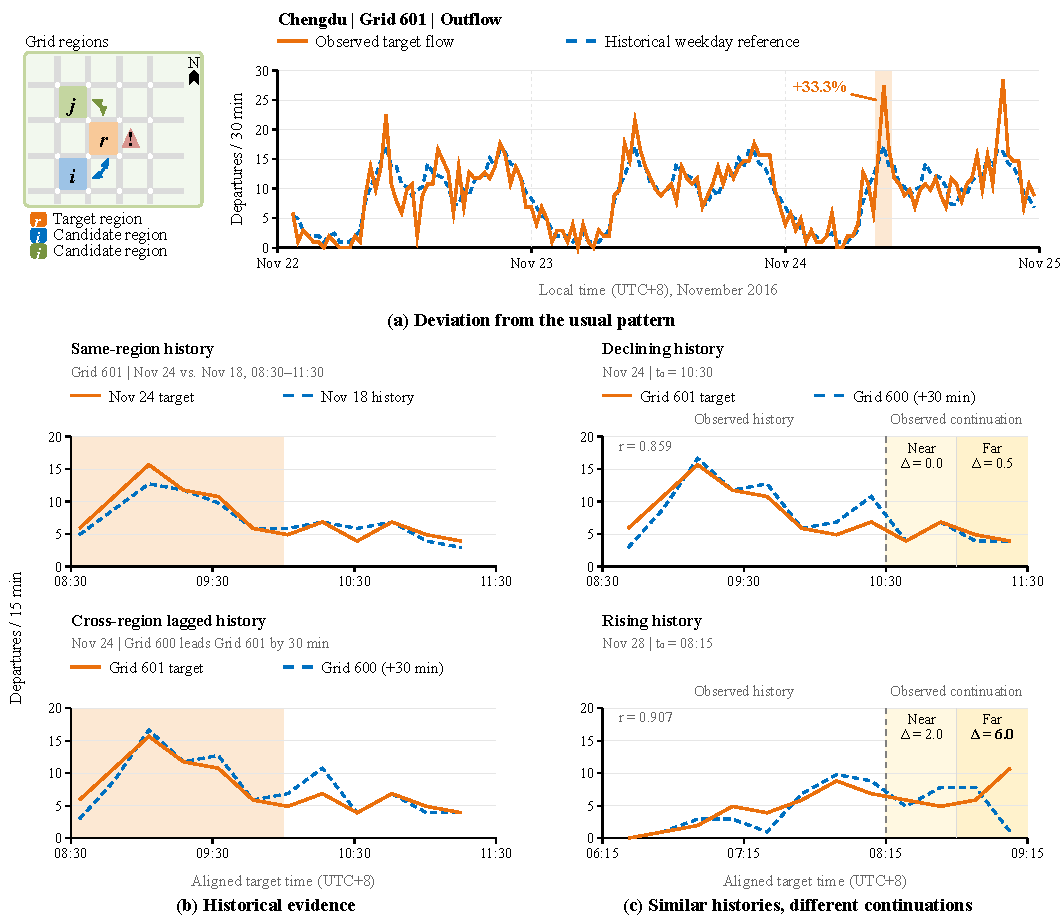
\includegraphics[width=\linewidth]{figures/introduction-case.pdf}
  \caption[常规流量模式偏离与历史信息关联的观测案例]{\textbf{常规流量模式偏离与历史信息关联的观测案例。} 成都2016年11月网格601的流出量，时间均为UTC+8。（a）实测流量与训练期14个工作日同一时段的中位数参照对比；11月24日08:30--10:00的累计流出量高出参照33.3\%，左侧为区域关系示意。（b）同区域11月18日的历史序列及邻网格600提前30分钟的观测；邻区曲线右移30分钟以对齐目标时间。（c）两个案例中，\(r\)为观测截点\(t_0\)前8个15分钟计数的目标与对齐邻区序列之间的Pearson相关系数；Near和Far分别表示\(t_0\)后\([0,30)\)与\([30,60)\)分钟，\(\Delta\)为各区间内两条实测曲线的平均绝对差。（a）按30分钟聚合，（b、c）按15分钟聚合，\(\Delta\)的单位为流出次数/15分钟。案例为事后选取，（c）的后续曲线均为实测观测而非模型预测，Far区间所用邻区源观测发生在\(t_0\)之后。}
  \label{fig:intro-case}
\end{figure}

第一个挑战来自预测证据的异质性。当目标区域偏离常规模式时，可用于修正预测的信息并非来源于单一机制，而是具有明显不同的时间和空间语义。有向时滞关联描述其他区域历史状态与目标区域之间的时间错位关系，而节点自身演化则刻画其局部连续性。这些信息并不是同一种时空依赖的不同强弱形式，而是对应不同的预测角色。若将它们统一压缩到同一种图传播或同一套时序编码中，模型虽然能够学习联合表征，却难以显式保留不同证据的功能差异，也难以进一步形成针对基础预测误差的定向补偿。因此，真正需要解决的问题不是简单地“融合更多信息”，而是如何依据不同证据的作用机制，为其配置差异化的时间编码与关系支持，并将这些信息组织为具有明确角色的预测修正。

第二个挑战在于跨区域历史信息的参考价值具有显著的条件依赖性。空间邻近或历史相关只能表明两个区域可能存在联系，却不能保证候选区域的任一历史状态都适用于当前预测。事实上，同一个候选区域在不同历史时滞、不同时间尺度下所呈现的模式，其参考价值可能明显不同；而在多步预测中，不同未来时距所需要的历史信息也并不完全一致。因此，跨区域建模不能只回答“哪些节点相关”，还需要进一步回答：在当前流量背景下，应从哪个候选区域、哪个历史时刻和哪个时间尺度提取信息，并针对不同预测步赋予多少权重。如果缺乏这种条件化选择机制，无关甚至不匹配的历史消息可能与有效证据同时进入聚合过程，从而削弱对异常变化的刻画能力。

上述两个问题共同指向本文关注的核心研究问题：当目标区域流量偏离其常规时段模式时，如何联合节点自身近期动态与跨区域历史证据，对基础预测进行分层、选择性的残差修正，从而改善短时多步交通流量预测？ 从这一角度看，本文所需的并不是一个更复杂的统一编码器，而是一种能够在已有时空表征之上，分别完成“证据组织”和“历史消息选择”的多级精炼机制。

为此，本文提出一种级联式多级时空残差网络（Cascaded Multi-level Spatio-temporal Residual Network，CMSRN），通过异质专家的自适应融合与背景条件化的历史消息选择，对基础预测进行互补的残差精炼。框架首先通过共享双频时空编码提取低频与高频表征，生成基础预测；随后，状态证据专家残差精炼模块（SERR）围绕节点自身演化和有向时滞关联构建差异化专家，并依据当前状态分配其修正贡献；背景条件跨区域消息选择模块（BCMS）利用目标与来源区域的低频背景，对高频历史消息进行预测步相关的联合选择。两模块分别读取共享表征，生成的修正量在预测端加性融合，共同完成区域流入与流出的短时多步预测。

本文的主要贡献总结如下：

\begin{enumerate}
	\def\labelenumi{\arabic{enumi}.}
	\item
	提出状态证据驱动的异质角色残差精炼模块 SERR。针对常规模式偏离时预测证据的异质性及其贡献分配问题，SERR 构建自身演化与有向时滞两类互补专家，分别刻画节点自身时序演化与跨区域滞后关联。模块结合共享双频表征、相对常规基线的趋势偏差及短时波动证据，通过状态条件门控，在节点和流量通道层面自适应融合自身预测相对于基础预测的残差与时滞专家的补充修正，并以全局可学习强度调节修正幅度，实现对基础预测的状态条件化精炼。
	\item
	提出背景条件化的联合历史消息选择模块BCMS。针对跨区域历史证据的参考价值随流量背景和预测时距变化的问题，BCMS利用目标区域与来源区域的低频背景调制高频多尺度模式匹配，在固定候选邻域内，针对不同预测步对“邻居---时滞---尺度”组合进行联合评分与加权聚合，使历史消息的选择同时适配双端流量背景与未来预测时距。通过将零消息选项纳入联合归一化，模块进一步自适应调节跨区域历史信息的总体引入程度，为基础预测提供背景条件化、预测步相关的残差补充。
	\item
	在成都和上海数据集上开展系统实验，验证CMSRN的预测性能与残差精炼效果。在与13种代表性基线的总体比较中，CMSRN在两城市的四项流入、流出预测任务上均取得最低AVG12 MAE，相较各任务最强基线降低0.46\%--2.00\%，并在其中三项任务上取得最低AVG12 RMSE。进一步结合独立重训练消融与常规模式偏离情景下的分组分析，考察两类残差通路的作用差异：固定模型诊断显示，自身演化修正在近期快速变化样本中具有更大的平均MAE收益，BCMS修正则在目标与候选区域的背景代理较接近时更有效，为角色化证据组织与背景条件化消息选择提供实验依据。
\end{enumerate}

% !TeX root = ../main.tex
% !TeX encoding = UTF-8
% !TeX spellcheck = none

% 原文此节部分引文编号与文末条目不对应，已保留；见 conversion-notes.md。
\section{相关工作}\label{sec:related-work}

\subsection{时空建模与频率解耦}\label{sec:frequency-related}

交通流预测的核心任务是在复杂空间依赖和动态时间变化之间建立有效映射。基于图神经网络的方法通过显式建模道路节点之间的关联关系，成为交通预测的重要研究方向。DCRNN 将交通状态传播建模为有向图上的扩散过程，并结合扩散卷积与循环神经网络捕获空间传播和时间演化规律 \cite{ref01}。STGCN 进一步将图卷积与时间卷积结合，实现高效的时空特征提取 \cite{ref02}。Graph WaveNet 通过自适应邻接矩阵学习潜在空间关系，并利用扩张时间卷积扩大时间感受野，从而突破预定义拓扑限制 \cite{ref03}。这些研究建立了交通预测中空间关系建模与时间序列编码的基本范式。

随后，研究者进一步从动态空间关系和多尺度交互角度增强时空建模能力。ASTGCN 和 GMAN 分别利用空间---时间注意力机制动态刻画节点间相关性，使模型能够关注不同时间和空间位置的重要信息 \cite{ref04,ref05}。MTGNN 和 AGCRN 通过数据驱动方式学习节点间关系，降低了对人工构建邻接矩阵的依赖 \cite{ref06,ref07}。STSGCN 和 STFGNN 则从时空同步建模以及多尺度时空融合角度进一步提升复杂交通模式的表达能力 \cite{ref08,ref09}。这些方法有效增强了空间依赖学习能力，但其核心仍主要围绕统一时空表示学习展开。

近年来，频率解耦方法进一步关注交通序列中不同时间动态的差异性。STWave利用小波分解将交通信号划分为不同频率成分，并分别学习其时空依赖关系，从而减少不同动态模式之间的相互干扰 \cite{ref10}。TEDDCF \cite{ref18}则进一步区分趋势分量与事件分量，并为低频趋势和高频事件设计独立的时间与空间编码路径 \cite{ref11}。这类方法表明，交通流中的稳定演化规律与快速变化模式具有不同的统计特征，需要通过差异化建模方式进行刻画。

然而，现有时空建模与频率解耦方法主要关注如何获得更具表达能力的基础时空表示，而对于当交通状态偏离常规模式后，如何利用不同来源的补充信息进一步修正预测结果仍缺少深入研究。

\subsection{异质证据与专家建模}\label{sec:experts-related}

交通流演化通常同时包含周期规律、趋势变化、局部扰动以及节点特定行为，因此利用不同结构组件刻画异质动态成为重要研究方向。ST-ResNet 将城市人群流动划分为时间邻近性、周期性和趋势性因素，并采用多个残差分支分别进行建模 \cite{ref12}。该方法证明了不同时间模式具有不同预测作用。

进一步地，部分研究开始探索通过解耦或专家机制显式区分不同交通动态。D2STGNN 通过解耦扩散信号与内在信号，使不同来源的交通变化能够分别建模，并增强模型对复杂动态的表达能力 \cite{ref13}。TESTAM 则设计时间专家、静态图专家和动态图专家，并通过专家路由机制根据输入状态选择不同专家组合，以适应交通动态变化 \cite{ref14}。

上述研究表明，交通预测中的不同动态因素具有不同作用机制，采用具有专门归纳偏置的结构能够提升模型对复杂交通模式的建模能力。然而，现有专家化方法主要关注如何根据输入状态选择或融合不同专家，其目标通常是获得更加灵活的整体表示，而不是围绕“预测修正”任务组织证据。

对于交通状态偏离常规模式的情境，关键问题并非简单判断使用哪个专家，而是明确不同预测证据承担的修正角色。例如，周期模式用于提供稳定参照，局部变化用于捕获短时扰动，有向时滞关系用于描述跨区域历史关联，而节点自身演化用于保持局部连续性。这些证据具有不同时间语义和空间关系，需要采用不同的处理路径。

\subsection{动态依赖与历史消息选择}\label{sec:messages-related}

除了异质时间模式建模外，交通预测还需要考虑空间关系随时间变化以及跨区域历史信息的有效利用。注意力机制为动态依赖学习提供了一种数据驱动方式。GMAN 通过空间注意力和时间注意力捕获节点间动态相关性，并利用转换注意力建立历史状态与未来预测之间的关联 \cite{ref15}。PDFormer 则进一步考虑交通传播过程中的时延因素，通过延迟感知特征变换建模动态长程空间依赖 \cite{ref16}。这些研究说明，交通关系不仅由空间距离决定，还受到时间对齐和传播延迟影响。

与此同时，自适应图学习方法进一步探索动态空间结构。MTGNN、AGCRN 等方法通过学习节点关系替代固定邻接矩阵，使模型能够捕获潜在空间关联 \cite{ref06,ref07}。然而，这类方法通常关注节点关系的生成或调整，而较少进一步区分：在当前交通背景和预测时距条件下，某一历史消息是否真正具有预测价值。

事实上，跨区域历史信息的有效性具有明显的条件依赖性。同一邻居区域可能在不同历史时滞、不同时间尺度以及不同预测步下表现出不同参考价值。因此，跨区域建模不仅需要回答“哪些区域相关”，还需要回答“哪些历史模式应该被选择，以及选择程度如何随预测目标变化”。

% !TeX root = ../main.tex
% !TeX encoding = UTF-8
% !TeX spellcheck = none

\section{问题定义}\label{sec:problem-definition}

将研究区域划分为\(N\)个规则网格，并将每个网格视为一个预测节点。记时刻\(t\)的区域流量矩阵为：
\begin{equation}
\label{eq:flow}
X_t = \bigl[x_t^{\mathrm{in}},\,x_t^{\mathrm{out}}\bigr]
\in \mathbb{R}^{N\times 2},
\end{equation}

其中，\(x_t^{\mathrm{in}},x_t^{\mathrm{out}}\in\mathbb{R}^{N}\)分别表示各节点在该采样时间段内的流入量与流出量，对应以该区域为目的地与出发地的出行计数。本文在同一模型中联合预测两类流量，通道顺序为流入、流出。以下序列张量按时间、节点、流量通道排列，并省略批次维度。

给定截至时刻\(t\)、长度为\(T\)的历史观测序列：
\begin{equation}
\label{eq:history}
X_{t-T+1:t} = \bigl[X_{t-T+1},\ldots,X_t\bigr]
\in \mathbb{R}^{T\times N\times 2},
\end{equation}

目标是联合预测未来\(H\)个时间步的流入量与流出量：
\begin{equation}
\label{eq:future}
Y_{t+1:t+H} = \bigl[X_{t+1},\ldots,X_{t+H}\bigr]
\in \mathbb{R}^{H\times N\times 2}.
\end{equation}

其中，\(T\)和\(H\)分别为历史窗口长度和预测步数。本文采用5分钟采样间隔，设置\(T=H=12\)，即利用过去60分钟的观测预测未来60分钟的流量。

上述任务可表示为学习时空映射：
\begin{equation}
\label{eq:mapping}
\widehat{Y}_{t+1:t+H}
= f_{\theta}\!\left(X_{t-T+1:t},C_t;\mathcal{S},\mathcal{B}\right)
\in \mathbb{R}^{H\times N\times 2},
\end{equation}

其中，\(\theta\)为模型的可学习参数；\(C_t\in\mathbb{R}^{T\times 2}\)为历史窗口对应的日内时刻与星期信息，在各节点间共享；\(\mathcal{S}\)表示预先构建的空间关系支持，包括节点自身关系、按流量通道构建的有向时滞关系及跨区域候选邻域；\(\mathcal{B}\)为训练期构建并固定使用的常规流量基线查找表。预测以截至\(t\)的观测及相应时间信息为依据，\(\widehat{Y}_{t+1:t+H}\)表示原始流量尺度上的预测结果。

为描述已观测交通状态对常规模式的偏离，对历史窗口内任一时刻\(u\in\{t-T+1,\ldots,t\}\)，从\(\mathcal{B}\)中提取对应的常规流量参照：
\begin{equation}
\label{eq:baseline}
b_u=\bigl[b_u^{\mathrm{in}},\,b_u^{\mathrm{out}}\bigr]
\in\mathbb{R}^{N\times 2}.
\end{equation}

该基线由训练期历史观测按节点、流量通道、工作日或周末类型及日内时段统计获得。相对于常规参照的流量偏差定义为：
\begin{equation}
\label{eq:deviation}
D_u=X_u-b_u\in\mathbb{R}^{N\times 2}.
\end{equation}

\(D_u\)量化已观测流量与对应常规水平之间的差异。方法学进一步介绍如何结合历史轨迹与常规参照构造趋势偏差和短时波动证据。

在上述流入与流出联合预测任务中，本文重点研究常规模式偏离时的预测修正：结合节点自身近期动态与跨区域时滞关联，自适应分配异质证据的修正贡献，并根据双端流量背景与预测时距选择历史消息。相应的残差精炼机制在第\ref{sec:methodology}节展开。

% !TeX root = ../main.tex
% !TeX encoding = UTF-8
% !TeX spellcheck = none

\section{方法学}\label{sec:methodology}

\subsection{总体框架}\label{sec:framework}

CMSRN 的整体架构如图~\ref{fig:cmsrn-architecture}所示。框架首先通过共享双频时空编码形成基础预测；SERR 利用自身演化与有向时滞两类专家组织修正证据，BCMS 根据双端流量背景与预测时距选择跨区域历史消息。两个模块分别读取共享表征、生成互补修正，并在预测端进行加性融合：
\begin{equation}
\label{eq:overall-prediction}
\widetilde{Y}=\widetilde{Y}^{0}+\Delta\widetilde{Y}^{S}+\Delta\widetilde{Y}^{B}.
\end{equation}
其中，\(\widetilde{Y}^{0}\)为基础预测，\(\Delta\widetilde{Y}^{S}\)和\(\Delta\widetilde{Y}^{B}\)分别为 SERR 与 BCMS 的修正，三者均属于\(\mathbb{R}^{H\times N\times2}\)。波浪号表示按流量通道标准化的预测量。下文将历史窗口内的位置重编号为\(k=1,\ldots,T\)，未来预测步记为\(h=1,\ldots,H\)，并用\(c\in\{\mathrm{in},\mathrm{out}\}\)区分流量通道。

\begin{figure}[!htbp]
  \centering
  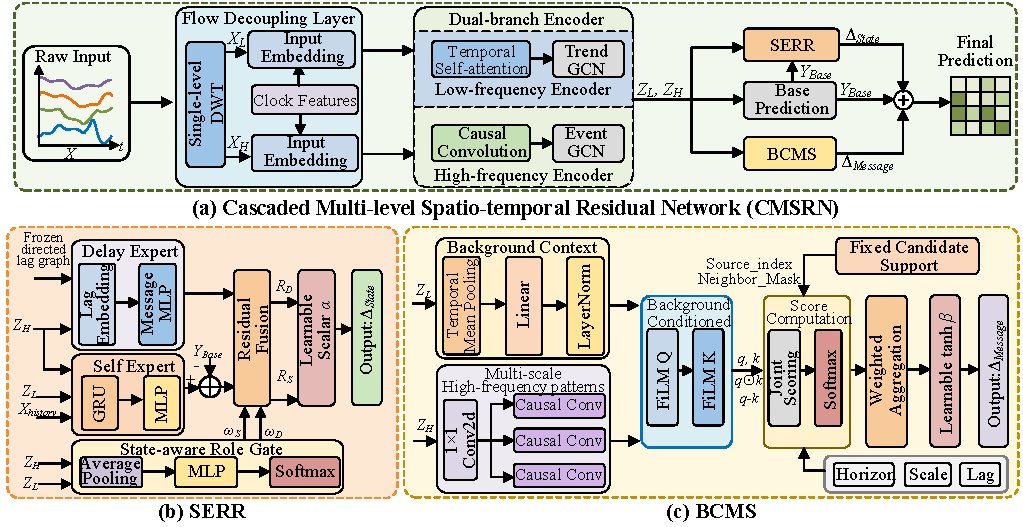
\includegraphics[width=\linewidth]{figures/model-architecture.pdf}
  \caption[CMSRN 的整体架构]{\textbf{CMSRN 的整体架构及核心模块。}（a）历史流量经单层小波分解与双分支时空编码形成低、高频表征，基础预测与 SERR、BCMS 产生的修正量在预测端融合。（b）SERR 通过自身演化专家、有向时滞专家及状态感知角色门控，生成角色相关的残差修正。（c）BCMS 利用低频背景调制高频多尺度模式匹配，针对不同预测步，对固定候选邻域内的邻居--时滞--尺度组合进行联合评分与加权聚合。图中的\(Y_{\mathrm{Base}}\)、\(\Delta\mathrm{State}\)和\(\Delta\mathrm{Message}\)分别对应\(\widetilde{Y}^{0}\)、\(\Delta\widetilde{Y}^{S}\)和\(\Delta\widetilde{Y}^{B}\)，均在标准化流量尺度下表示。}
  \label{fig:cmsrn-architecture}
\end{figure}

\subsection{共享双频时空表征}\label{sec:dual-frequency}

为区分平缓变化与短时波动，CMSRN 采用 TEDDCF~\cite{ref18}的低、高频双分支结构提取共享表征。首先，沿历史窗口的时间维对各流量通道进行单层离散小波分解与重构，得到低频和高频序列。两类序列均使用训练期流量的逐通道均值与标准差进行标准化，再附加日内时刻与星期信息，形成\(U_L,U_H\in\mathbb{R}^{T\times N\times4}\)。两分支共享输入投影与时间嵌入，随后分别执行低频时间自注意力及趋势图编码、高频时间卷积及事件图编码：
\begin{equation}
\label{eq:low-frequency}
Z_L=\mathrm{F}_L(U_L),
\end{equation}
\begin{equation}
\label{eq:high-frequency}
Z_H=\mathrm{F}_H(U_H),
\end{equation}
其中，\(Z_L,Z_H\in\mathbb{R}^{T\times N\times d_b}\)，\(d_b\)为共享表征维度。基础预测由两类特征融合后获得：
\begin{equation}
\label{eq:base-prediction}
\widetilde{Y}^{0}=\mathrm{R}\!\left(\operatorname{ReLU}\!\left[Z_L+\operatorname{GLU}(Z_L)+Z_H\right]\right).
\end{equation}
\(\mathrm{R}\)为覆盖完整历史窗口的卷积预测头，将特征映射为未来\(H\)步的流入与流出预测。SERR 和 BCMS 使用的\(Z_L\)取自 GLU 之前，与\(Z_H\)共同作为共享输入。

\subsection{状态证据驱动的异质角色残差精炼}\label{sec:serr}

SERR 按照节点自身演化与跨区域时滞关联组织两类互补专家，并根据当前状态分配其修正贡献，如图~\ref{fig:cmsrn-architecture}（b）所示。为连接常规参照与近期动态，记\(x_{k,i,c}\)为历史位置\(k\)处节点\(i\)的通道\(c\)原始流量，\(b_{k,i,c}\)为对应的训练期常规基线。状态证据定义为：
\begin{equation}
\label{eq:state-evidence}
\begin{aligned}
\bar{x}_{k,i,c}&=\frac{1}{\ell_k}\sum_{r=k-\ell_k+1}^{k}x_{r,i,c},\qquad \ell_k=\min(3,k),\\
e_{i,c}&=\left[\bar{x}_{T,i,c}-b_{T,i,c},\;x_{T,i,c}-\bar{x}_{T,i,c}\right]^{\mathsf T}.
\end{aligned}
\end{equation}
\(e_{i,c}\in\mathbb{R}^{2}\)分别描述末时刻的趋势偏差与短时波动。均值仅使用当前历史窗口内已观测的位置，窗口起始处按可用长度计算。

自身演化专家在各节点内编码近期轨迹。对于每个流量通道，将共享双频特征之和与原始流量拼接，输入共享 GRU，并将末隐藏状态映射为多步预测：
\begin{equation}
\label{eq:self-expert}
P^{\mathrm{self}}_{:,i,c}
=\mathcal{P}_{S}\!\left(\psi_S\!\left(\operatorname{GRU}_{\mathrm{last}}
\left([Z_{L,k,i}+Z_{H,k,i}\,\Vert\,x_{k,i,c}]_{k=1}^{T}\right)\right)\right).
\end{equation}
其中，\(\Vert\)表示特征拼接，\(\psi_S\)为含 Tanh 激活的两层感知机，\(\mathcal{P}_S\)将\(d_b\)维特征线性映射为\(H\)步预测。该分支在共享时空表征上进一步提取节点自身的时间演化信息。

有向时滞专家从预先构建并冻结的关系集合\(\mathcal{E}_c\)中提取来源节点历史特征。对边\((j,i,\ell)\in\mathcal{E}_c\)，\(j\)为来源节点，\(i\)为目标节点，\(\ell\)为满足\(0<\ell<T\)的历史时滞。来源高频特征经滞后嵌入调制，并结合目标状态证据转换为补充消息：
\begin{equation}
\label{eq:delay-expert}
\begin{aligned}
\eta_{i,c}&=W_e e_{i,c},\\
m_{j\to i,\ell,c}&=\psi_D\!\left([(1+\tanh v_{\ell})\odot Z_{H,T-\ell,j}\,\Vert\,\eta_{i,c}]\right),\\
R^{\mathrm{delay}}_{:,i,c}&=\mathcal{P}_D\!\left(\eta_{i,c}
+\sum_{(j,i,\ell)\in\mathcal{E}_c}a_{ji\ell}^{c}m_{j\to i,\ell,c}\right).
\end{aligned}
\end{equation}
这里，\(W_e\in\mathbb{R}^{d_b\times2}\)为证据投影，\(v_\ell\in\mathbb{R}^{d_b}\)为可学习滞后嵌入，\(\psi_D\)为含 SiLU 激活的无偏置消息变换，\(a_{ji\ell}^{c}\)为固定边权，\(\mathcal{P}_D\)为多步线性输出头。两类专家各自的参数在节点和流量通道间共享，有向时滞关系按流量通道分别给定。

状态条件门控利用低、高频特征的时间均值及两类流量的状态证据，确定专家贡献：
\begin{equation}
\label{eq:role-gate}
\Omega_i=\operatorname{Softmax}_{\mathrm{expert}}\!\left(
\operatorname{reshape}_{2\times2}\,g\!\left(
[\bar{Z}_{L,i}\,\Vert\,\bar{Z}_{H,i}\,\Vert\,e_{i,\mathrm{in}}\,\Vert\,e_{i,\mathrm{out}}]
\right)\right).
\end{equation}
\(\bar{Z}_{L,i},\bar{Z}_{H,i}\)为沿历史时间维求均值得到的\(d_b\)维向量，\(g\)为含 SiLU 激活的两层感知机。\(\Omega_i\in\mathbb{R}^{2\times2}\)的行对应流量通道，列对应自身与时滞专家，Softmax 在专家维归一化，得到\(\omega^S_{i,c}\)和\(\omega^D_{i,c}\)。这些权重随样本、节点与流量通道变化，并在全部预测步间共享。最终修正为：
\begin{equation}
\label{eq:serr-residual}
\Delta\widetilde{Y}^{S}_{h,i,c}
=\alpha\left[\omega^S_{i,c}\left(P^{\mathrm{self}}_{h,i,c}-\widetilde{Y}^{0}_{h,i,c}\right)
+\omega^D_{i,c}R^{\mathrm{delay}}_{h,i,c}\right].
\end{equation}
\(P^{\mathrm{self}}\)与\(R^{\mathrm{delay}}\)均对应基础预测所在的标准化流量尺度，\(\alpha\)为全局可学习标量。自身专家通过相对于基础预测的残差参与修正，时滞专家则提供跨区域历史信息的补偿，两者由状态条件门控协同融合。

\subsection{背景条件化的联合历史消息选择}\label{sec:bcms}

BCMS 在固定候选邻域内，依据当前背景及未来预测时距选择历史消息，如图~\ref{fig:cmsrn-architecture}（c）所示。首先，将低频特征的时间均值映射为节点背景，并对高频特征提取多尺度模式：
\begin{equation}
\label{eq:bcms-context-pattern}
\xi_i=\operatorname{LN}\!\left(\mathcal{P}_b(\bar{Z}_{L,i})\right),
\qquad z^s=\mathcal{T}_s\!\left(\mathcal{P}_H(Z_H)\right).
\end{equation}
\(\xi_i\in\mathbb{R}^{d}\)，\(z^s\in\mathbb{R}^{T\times N\times d}\)，其中\(d=32\)。\(\mathcal{P}_b\)为线性投影，\(\mathcal{P}_H\)为各尺度共享的\(1\times1\)卷积。\(\mathcal{T}_s\)由左侧填充的深度时间卷积、逐点卷积和 GELU 构成；三个尺度采用大小为3的卷积核及扩张率1、2、4，对应时间覆盖范围\(r_s\in\{3,5,9\}\)。

记节点\(i\)的固定候选来源集合为\(\mathcal{N}_i\)，历史时滞\(\tau\in\{0,1,2,3\}\)。有效候选集合为\(\mathcal{A}_i=\{(j,\tau,s):j\in\mathcal{N}_i,\ r_s+\tau\leq T\}\)，其中每个节点至多保留8个来源。对同一尺度上的目标末时刻模式与来源历史模式，分别使用双端低频背景调制查询和键：
\begin{equation}
\label{eq:background-conditioned-qk}
\begin{aligned}
q_i^s&=(1+\gamma_q(\xi_i))\odot Q(z^s_{T,i})+\delta_q(\xi_i),\\
k_{j,\tau}^s&=(1+\gamma_k(\xi_j))\odot K(z^s_{T-\tau,j})+\delta_k(\xi_j).
\end{aligned}
\end{equation}
\(Q,K\)为可学习仿射映射，\(\gamma\)和\(\delta\)分别产生\(d\)维缩放与平移参数。由此，高频模式的匹配同时受目标与来源区域的低频背景约束。

对于预测步\(h\)，联合评分定义为：
\begin{equation}
\label{eq:joint-message-score}
\begin{aligned}
u_{i,j,\tau,s}
&=A_q q_i^s+A_k k_{j,\tau}^s
+A_p(q_i^s\odot k_{j,\tau}^s)+A_d(q_i^s-k_{j,\tau}^s)+b_a,\\
a_{h,i,j,\tau,s}
&=w_a^{\mathsf T}\operatorname{GELU}\!\left(
u_{i,j,\tau,s}+e_{\mathrm{lag}}(\tau)+e_{\mathrm{scale}}(r_s)+e_{\mathrm{hor}}(h)\right).
\end{aligned}
\end{equation}
其中，\(A_q,A_k,A_p,A_d\in\mathbb{R}^{d\times d}\)，\(b_a,w_a\in\mathbb{R}^{d}\)为可学习参数。三类时间编码分别对\([v,\sin(2\pi v),\cos(2\pi v)]^{\mathsf T}\)进行无偏置线性投影，\(v\)为相应时滞、尺度覆盖范围或预测时距换算得到的小时数。预测步编码在非线性评分之前引入，使候选贡献随未来时距变化。

为调节历史信息的总体引入程度，在每个预测步的候选集合中加入分数和值均为零的消息选项。对真实候选，联合归一化权重为：
\begin{equation}
\label{eq:joint-message-softmax}
w_{h,i,j,\tau,s}
=\frac{\exp(a_{h,i,j,\tau,s})}
{1+\displaystyle\sum_{(j',\tau',s')\in\mathcal{A}_i}\exp(a_{h,i,j',\tau',s'})}.
\end{equation}
分母中的1对应零消息，其占据的概率质量允许降低真实历史消息的总权重。来源高频模式经值投影后加权聚合，并生成双通道修正：
\begin{equation}
\label{eq:bcms-residual}
\begin{aligned}
m_{h,i}&=\sum_{(j,\tau,s)\in\mathcal{A}_i}
w_{h,i,j,\tau,s}W_vz^s_{T-\tau,j},\\
\Delta\widetilde{Y}^{B}_{h,i,:}&=\tanh(\beta)\,W_o m_{h,i}.
\end{aligned}
\end{equation}
\(W_v\in\mathbb{R}^{d\times d}\)与\(W_o\in\mathbb{R}^{2\times d}\)均为无偏置投影，\(\beta\)为全局可学习标量。流入与流出共享消息选择权重和聚合表示，由双输出头形成对应修正。BCMS 的权重针对每个预测步生成，与 SERR 在预测步间共享的专家权重形成互补。

\subsection{联合预测输出}\label{sec:joint-output}

将两类修正按式~\eqref{eq:overall-prediction}叠加至基础预测后，使用训练期输入窗口估计并固定的逐通道统计量恢复原始流量尺度：
\begin{equation}
\label{eq:inverse-scaling}
\widehat{Y}_{t+h,i,c}
=\sigma_c\left(\widetilde{Y}^{0}_{h,i,c}
+\Delta\widetilde{Y}^{S}_{h,i,c}+\Delta\widetilde{Y}^{B}_{h,i,c}\right)+\mu_c.
\end{equation}
其中，\(\mu_c\)和\(\sigma_c\)分别为通道\(c\)的均值与标准差。两个全局强度参数\(\alpha\)和\(\beta\)均初始化为零，因此初始输出与基础预测一致；SERR 门控末层同时采用零初始化，使两类专家初始权重均为0.5。模型由此在统一的流入与流出预测目标下学习两条互补修正通路的贡献。


% !TeX root = ../main.tex
% !TeX encoding = UTF-8
% !TeX spellcheck = none
\section{实验与分析}\label{sec:experiments}

\subsection{实验设置}\label{sec:exp-settings}

\subsubsection{数据集、预处理和预测协议}\label{sec:exp-datasets}

我们在成都和上海两个区域流量数据集上开展实验，分别由2016年11月的成都滴滴网约车订单和2016年8月的上海出租车OD记录构建。每个城市采用固定核心区域，并划分为\(32\times32\)个规则网格，以5分钟为时间间隔统计流量。订单目的地端点按到达时刻计入所在网格的流入量，起点端点按出发时刻计入流出量，两类端点独立聚合。因此，本文的区域流量表示出行到达与出发的端点计数。图~\ref{fig:chengdu-t5-dataset}和图~\ref{fig:shanghai-t5-dataset}展示两城市的端点分布、核心区域网格及平均流量分布，表~\ref{tab:dataset-summary}汇总数据属性与样本规模。

数据预处理统一采用北京时间。首先删除完全重复及时间或坐标无效的记录，再保留出行时长为2--120分钟、起终点位于城市粗边界内且平均速度不超过\(120\,\mathrm{km/h}\)的订单，其中平均速度由起终点球面距离与出行时长计算。随后，将落入核心区域和观测时段的端点聚合至相应网格与时间片；来源正常且无端点事件的位置记为零。清洗后，成都和上海分别保留6,082,753和7,744,423条订单。两城市的完整时间轴分别包含8,640和8,928个时间片，每个时间片对应1,024个网格的流入与流出计数。

\begin{table}[!htbp]
  \centering
  \caption{数据集属性与窗口级划分规模}
  \label{tab:dataset-summary}
  \small
  \begin{tabular}{lcc}
    \toprule
    属性 & 成都 & 上海 \\
    \midrule
    观测时段 & 2016-11-01至2016-11-30 & 2016-08-01至2016-08-31 \\
    网格数 & \(32\times32\) & \(32\times32\) \\
    单网格近似尺寸（km） & \(0.42\times0.44\) & \(0.80\times0.68\) \\
    采样间隔 & 5分钟 & 5分钟 \\
    完整时间片数 & 8,640 & 8,928 \\
    清洗后订单数 & 6,082,753 & 7,744,423 \\
    \bottomrule
  \end{tabular}
  \par\smallskip
\end{table}

预测采用步长为1的连续滑动窗口，以过去12步（60分钟）的观测联合预测未来12步（5--60分钟）的流入与流出，并保留历史窗口对应的日内时段与星期信息。窗口按预测起点的时间顺序，以约\(60\%\)、\(20\%\)和\(20\%\)划分为训练集、验证集与测试集，各方法使用相同的固定划分索引。

模型仅在已观测历史窗口内构造双频输入，并利用训练样本的历史记录分别估计流入与流出通道的均值和标准差，对低、高频输入应用同一组通道统计量。验证和测试阶段沿用固定统计量，预测经逐通道逆标准化恢复至原始流量尺度。常规流量基线及关系支持由训练期数据预先构建并固定，状态证据在预测时由已观测历史生成。

\begin{figure}[!htbp]
  \centering
  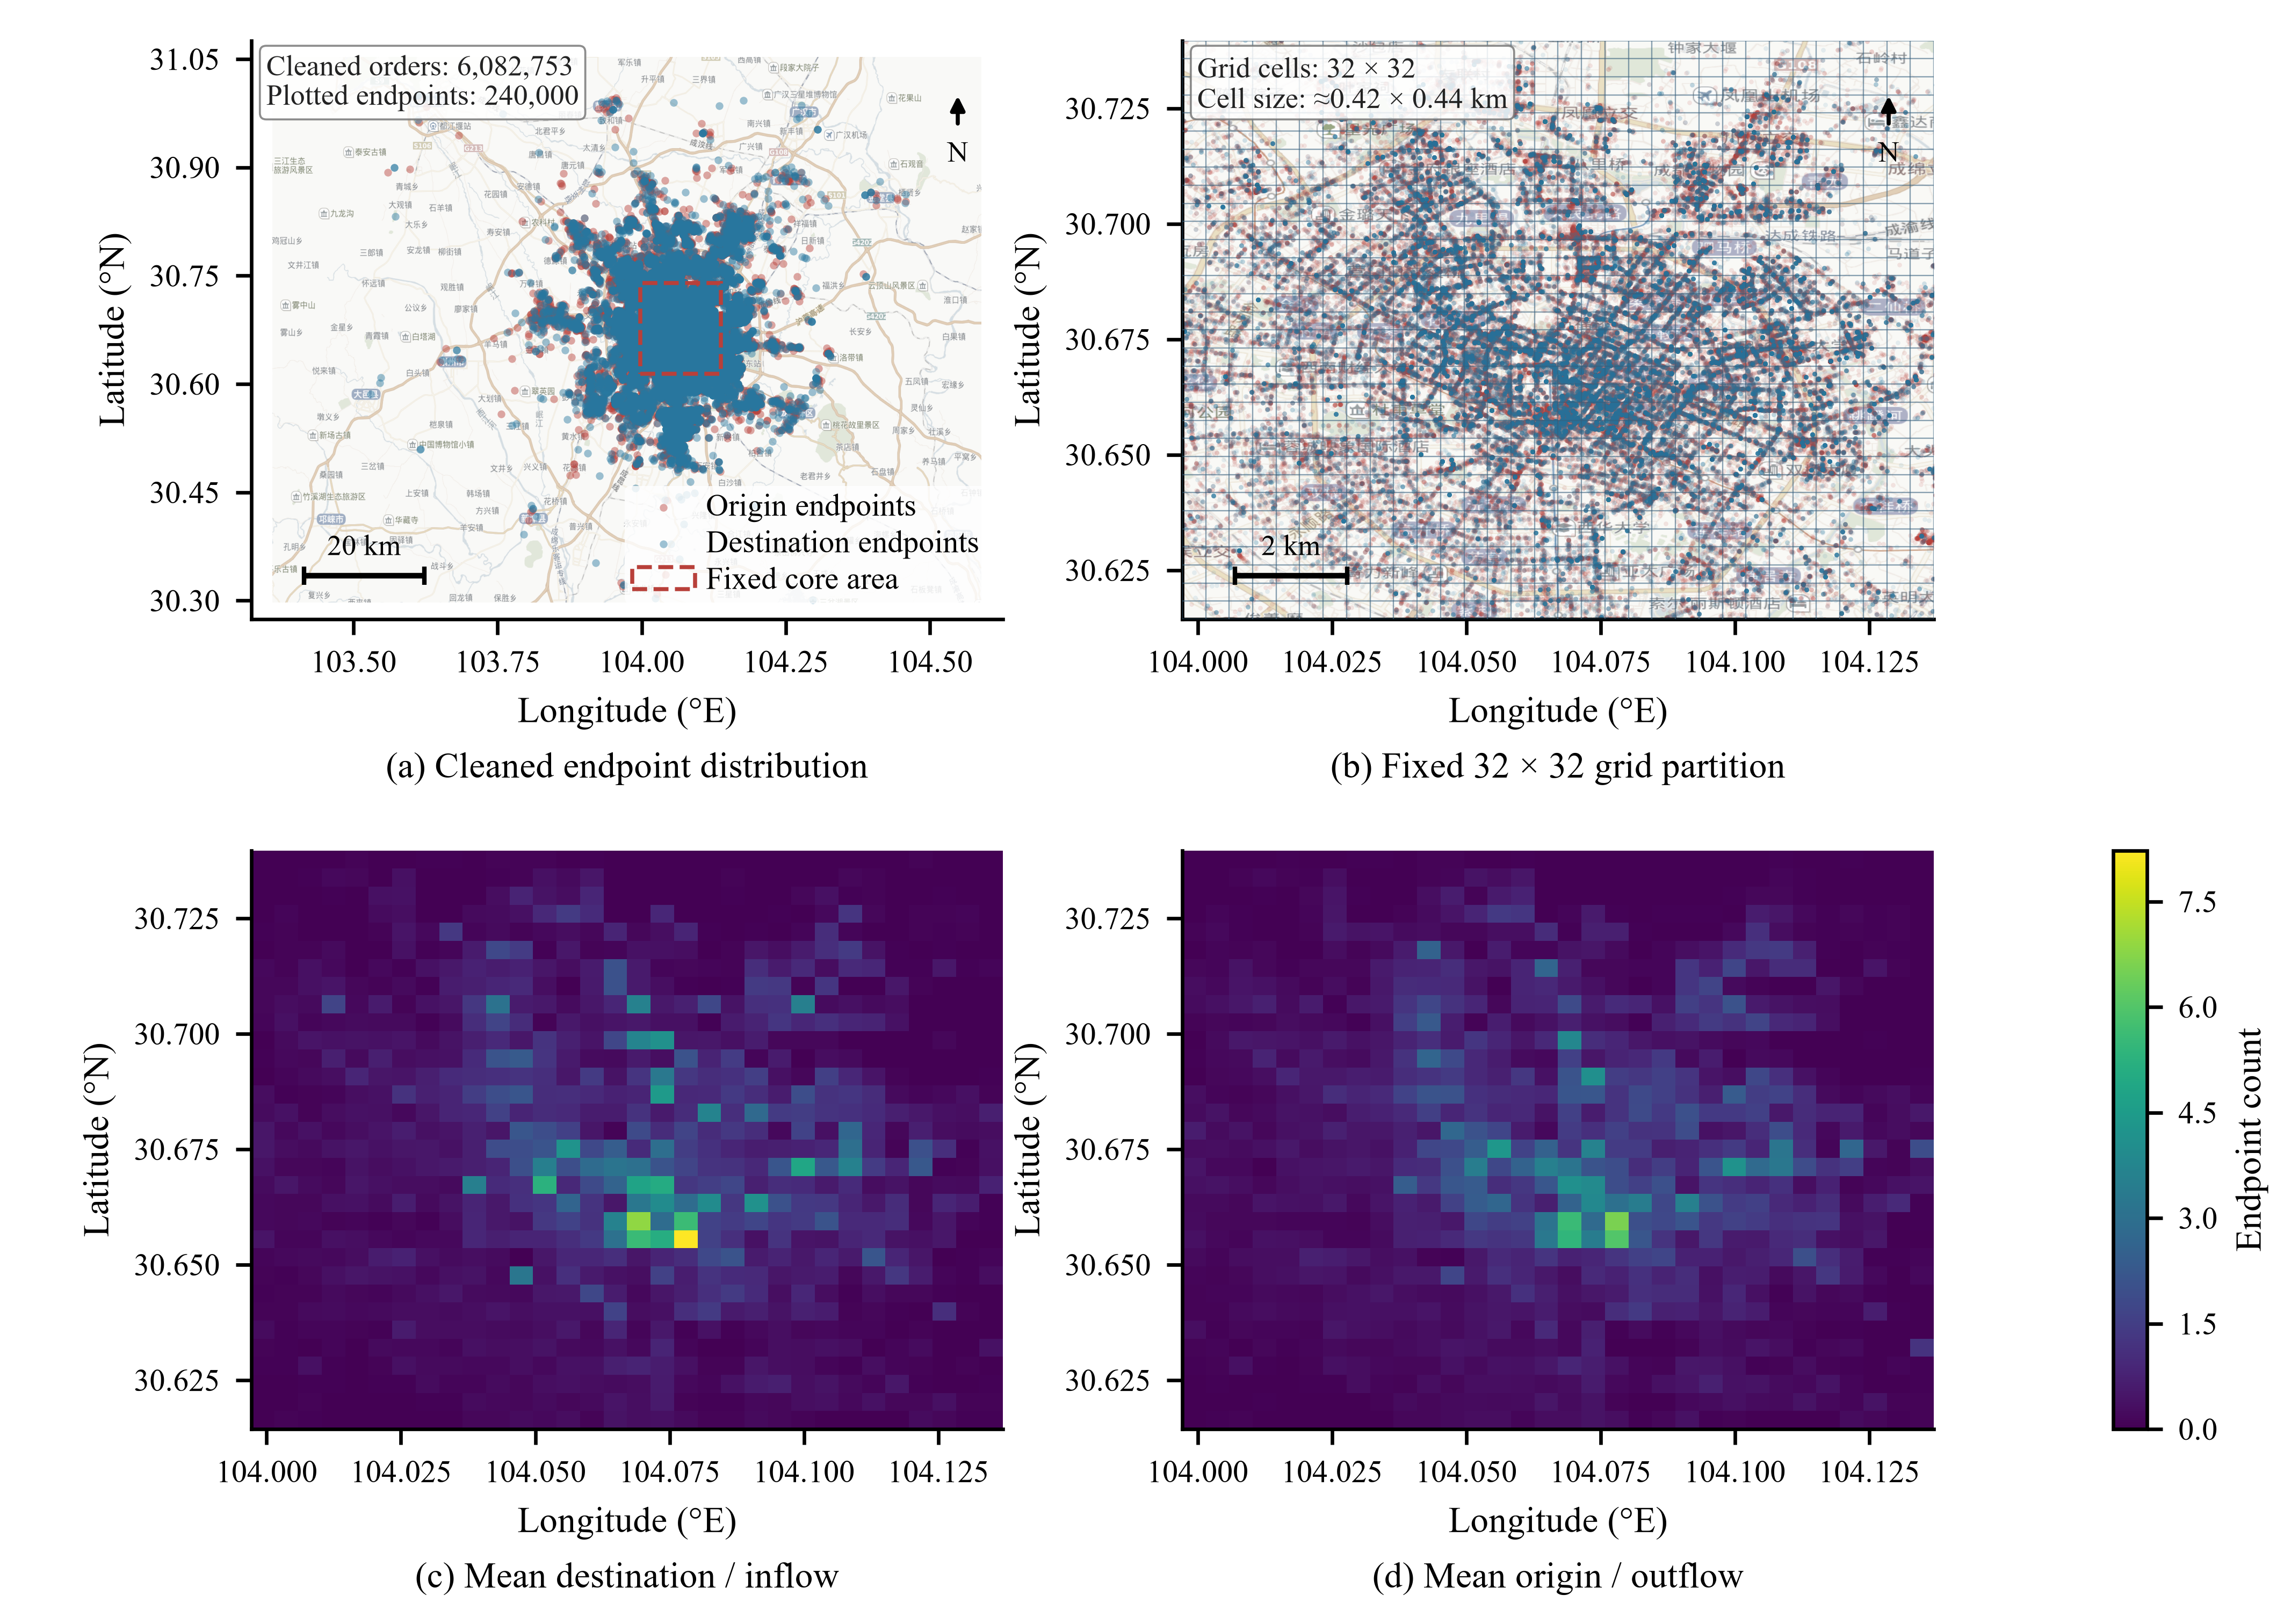
\includegraphics[width=\linewidth]{figures/chengdu-t5-overview.png}
  \caption[成都数据集的空间分布]{\textbf{成都数据集的空间分布与网格划分。}（a）清洗后订单的抽样起终点分布，虚线框标出固定核心区域。（b）核心区域内的\(32\times32\)网格。（c）平均目的地端点计数，对应流入量。（d）平均起点端点计数，对应流出量。均值基于来源质量正常的5分钟时间片计算。}
  \label{fig:chengdu-t5-dataset}
\end{figure}

\begin{figure}[!htbp]
  \centering
  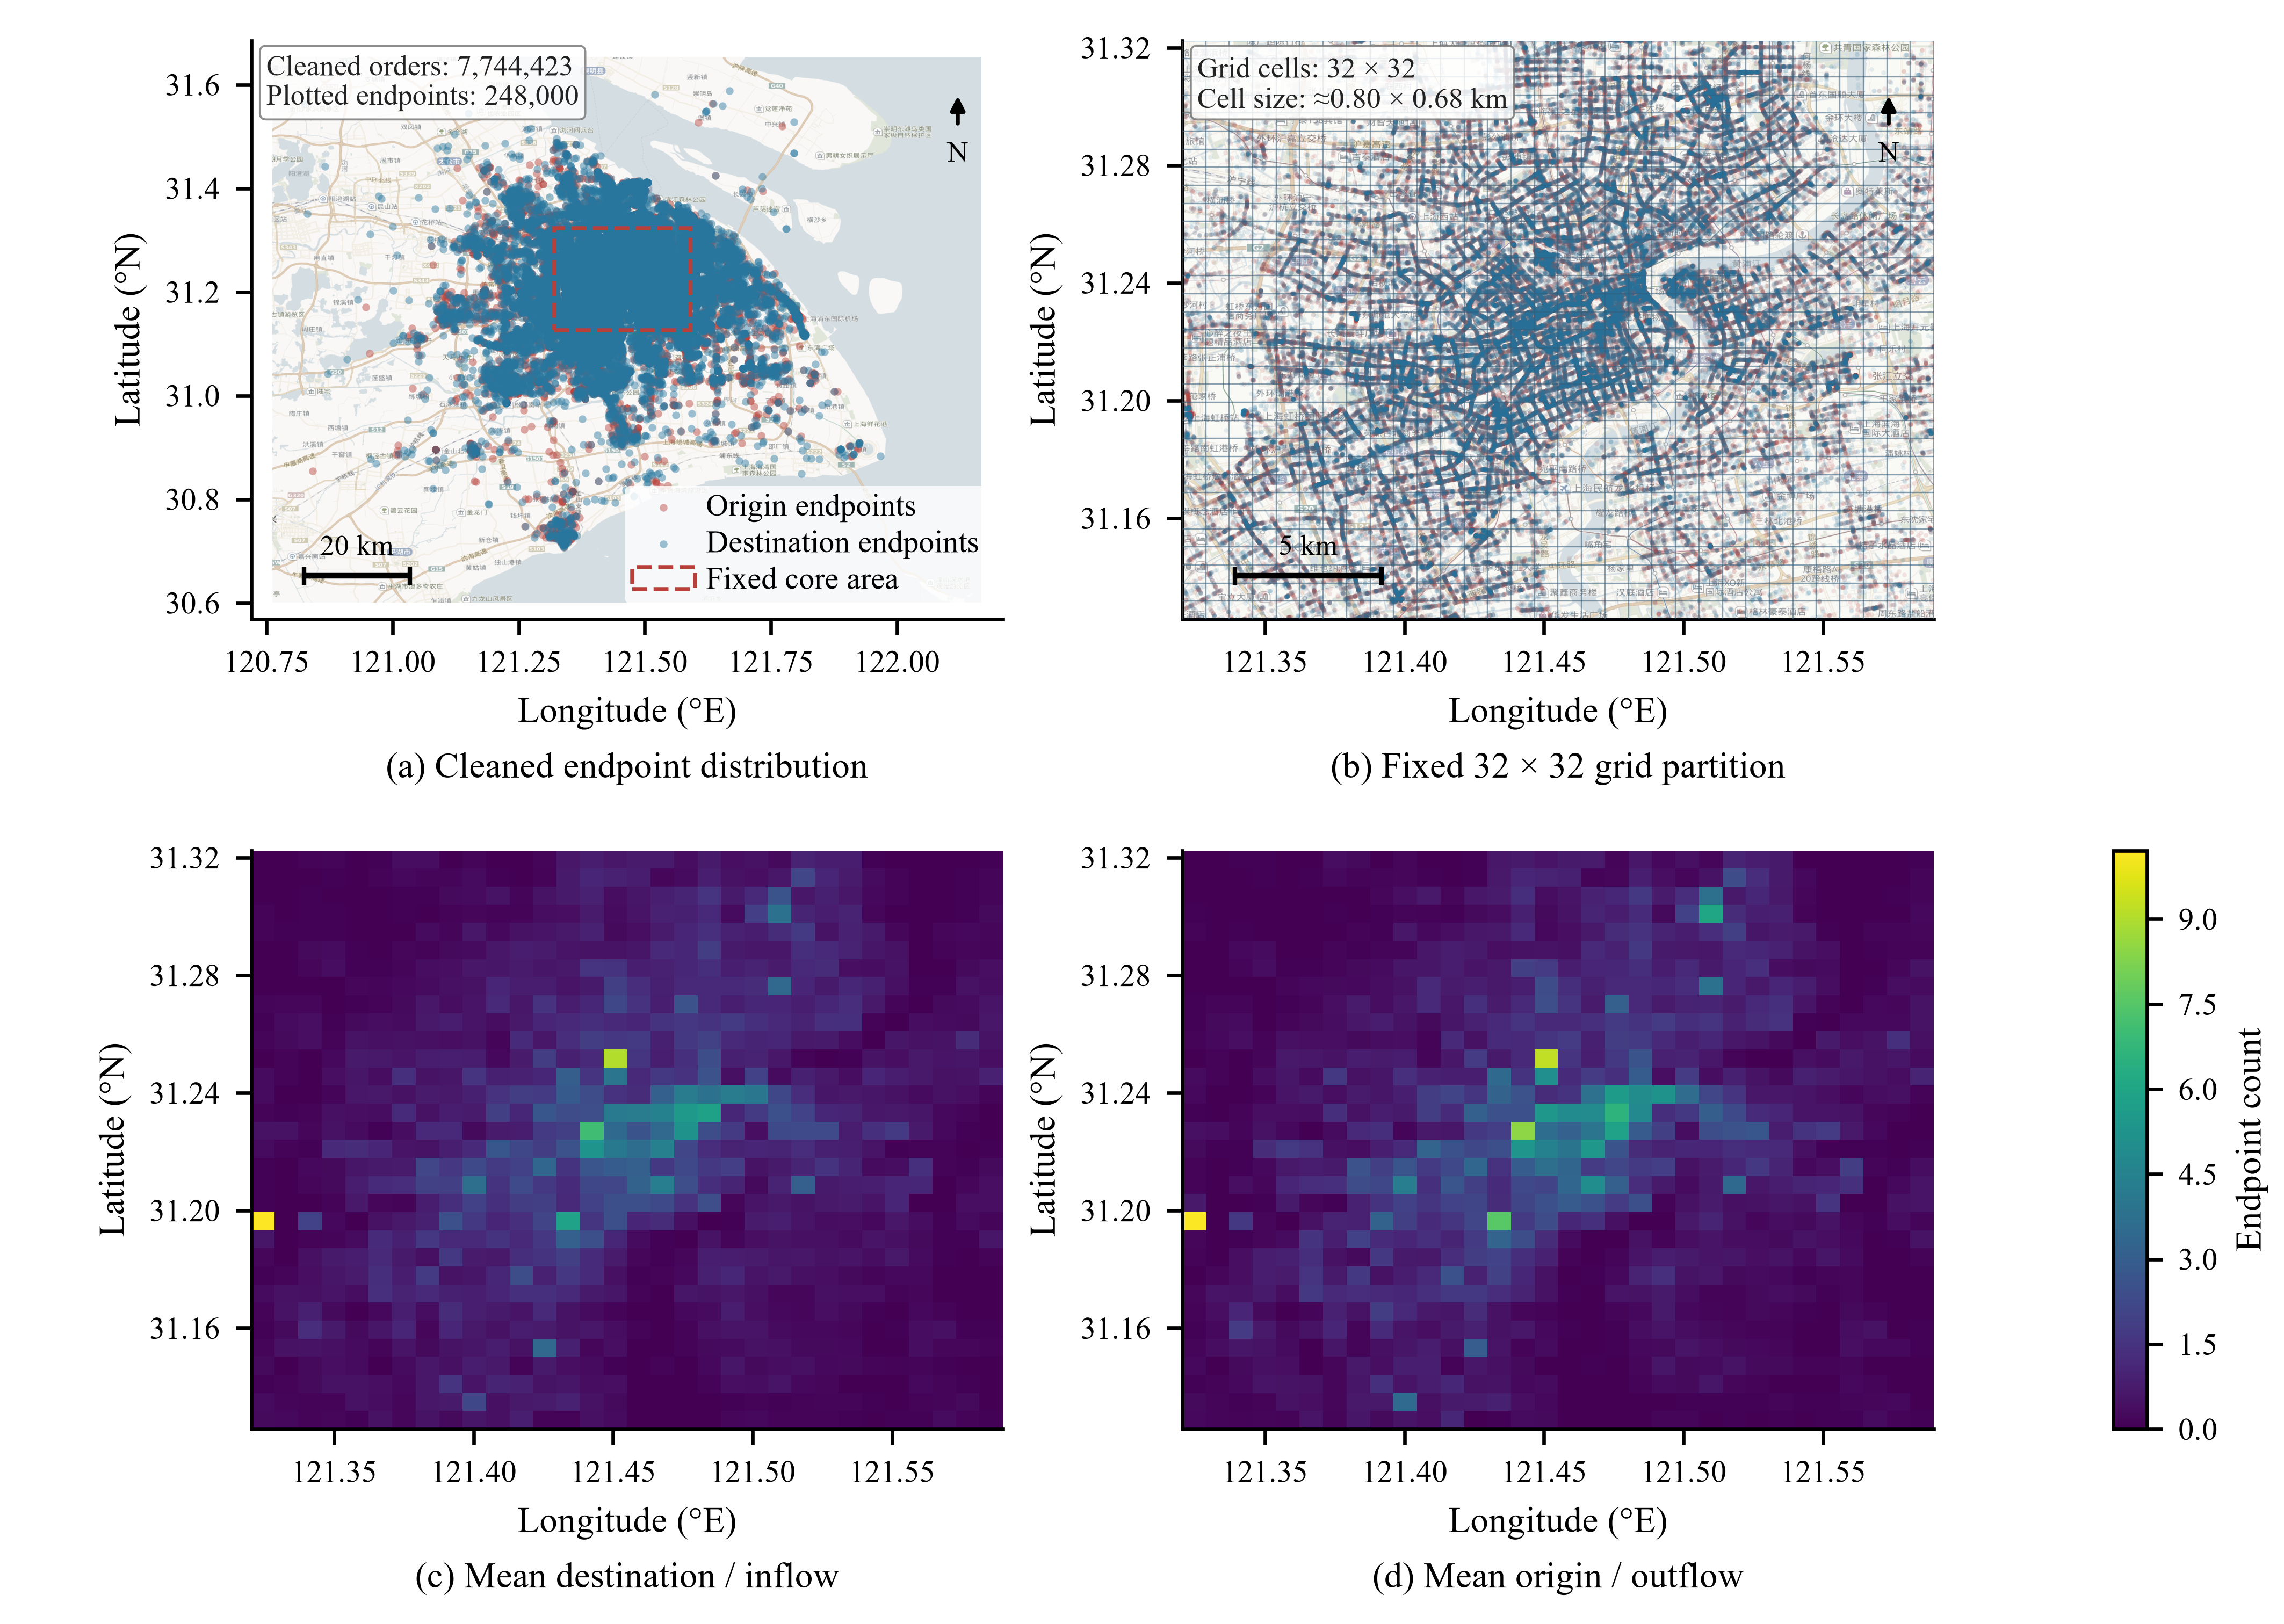
\includegraphics[width=\linewidth]{figures/shanghai-t5-overview.png}
  \caption[上海数据集的空间分布]{\textbf{上海数据集的空间分布与网格划分。}（a）清洗后订单的抽样起终点分布，虚线框标出固定核心区域。（b）核心区域内的\(32\times32\)网格。（c）平均流入量。（d）平均流出量。均值统计排除2016年8月11--14日的采集异常区间；端点散点图采用全月清洗订单的逐日抽样。}
  \label{fig:shanghai-t5-dataset}
\end{figure}

\subsubsection{基线和评估指标}\label{sec:exp-baselines-metrics}

主要对比实验选取13种基线方法与CMSRN进行比较，覆盖三类预测范式。传统方法包括历史平均（HA）和支持向量回归（SVR）。交通预测深度模型包括DCRNN~\cite{ref01}、STGCN~\cite{ref02}、Graph WaveNet（GWNet）\cite{ref03}、DSTAGNN~\cite{ref19}、PDFormer~\cite{ref10}、STDN~\cite{ref20}、MetaDG~\cite{ref21}、HyperD~\cite{ref22}和RAST~\cite{ref23}，涵盖图结构学习、动态时空依赖、序列分解与历史信息检索等建模思路。通用时间序列模型包括PatchTST~\cite{ref12}和TimeMixer~\cite{ref13}。各方法采用第\ref{sec:exp-datasets}节的固定时间划分和12步预测任务，在成都和上海数据集上分别评价流入与流出。

针对常规模式偏离的扩展情景比较（第\ref{sec:scenario-performance}节），另加入向量自回归（VAR）、STNorm~\cite{ref24}和STWave~\cite{ref11}。三者分别补充线性多变量建模、时空归一化与频率解耦方法。第\ref{sec:exp-main-results}节结果表的排名范围为原有13种基线，情景分析的排名范围为扩展后的16种基线。

评价指标采用平均绝对误差（MAE）和均方根误差（RMSE），均在原始流量尺度上计算。设\(\mathcal{T}_{\mathrm{test}}\)为测试窗口的预测起点集合，\(y_{t,h,i,c}\)和\(\widehat y_{t,h,i,c}\)分别为预测起点\(t\)、预测步\(h\)、网格\(i\)及流量通道\(c\in\{\mathrm{in},\mathrm{out}\}\)对应的真实值与预测值，误差记为\(e_{t,h,i,c}=\widehat y_{t,h,i,c}-y_{t,h,i,c}\)。采用正目标值掩码，对每个预测步和流量通道定义有效位置集合
\[
\Omega_{h,c}=\bigl\{(t,i)\mid t\in\mathcal{T}_{\mathrm{test}},\ 1\leq i\leq N,\ y_{t,h,i,c}>0\bigr\}.
\]
在全部测试窗口与节点的有效位置上合并计算
\begin{equation}
  \label{eq:eval-mae}
  \mathrm{MAE}_{h,c}
  =\frac{1}{|\Omega_{h,c}|}
    \sum_{(t,i)\in\Omega_{h,c}}|e_{t,h,i,c}|,
\end{equation}
\begin{equation}
  \label{eq:eval-rmse}
  \mathrm{RMSE}_{h,c}
  =\sqrt{\frac{1}{|\Omega_{h,c}|}
    \sum_{(t,i)\in\Omega_{h,c}}e_{t,h,i,c}^{2}}.
\end{equation}
其中，\(|\Omega_{h,c}|\)为有效位置数量，测试批次补齐产生的重复样本不参与统计。流入与流出的有效位置和指标分别计算，两项指标均以较小值表示较低预测误差。

我们报告H3、H6和H12三个单步结果，分别对应第3、6和12个预测步，即15、30和60分钟预测时距。同时，以AVG12表示全部12个单步指标的算术平均：
\begin{equation}
  \label{eq:eval-avg12}
  \mathrm{AVG12}\text{-}\mathcal{M}_{c}
  =\frac{1}{12}\sum_{h=1}^{12}\mathcal{M}_{h,c},
  \qquad\mathcal{M}\in\{\mathrm{MAE},\mathrm{RMSE}\}.
\end{equation}
其中，AVG12的RMSE先在各预测步内计算，再跨步取平均。上述汇总方式同时反映不同预测时距的表现与整个预测区间的平均误差。


% !TeX root = ../main.tex
% !TeX encoding = UTF-8
% !TeX spellcheck = none
\subsection{主要实验结果}\label{sec:exp-main-results}

本节从总体预测精度、空间分布、常规模式偏离情景及残差作用四个方面评价CMSRN，结合全测试集比较与固定模型诊断，考察两类修正证据在不同交通状态下的表现。

\subsubsection{整体预测性能}\label{sec:results-overall}

表~\ref{tab:chengdu-inflow}--\ref{tab:shanghai-outflow}比较了CMSRN与13种基线在成都和上海流入、流出预测任务上的表现。在上述13种基线的比较范围内，CMSRN在32个表列指标中取得26项最优，其余6项均排名第二；在反映整个预测区间表现的8项AVG12指标中，取得7项最优。以下相对变化均根据未舍入数值计算，并以对应任务和指标的最强基线为参照。

CMSRN在两个城市的流入与流出任务上均取得最低AVG12 MAE。成都流入和流出的AVG12 MAE分别为0.708和0.709，相较于HyperD分别降低2.00\%和0.46\%；上海流入和流出的对应结果为0.728和0.774，分别降低1.19\%和0.46\%。

RMSE呈现出更明显的任务差异。成都流入、成都流出和上海流入的AVG12 RMSE分别为1.294、1.223和1.228，相较于各自最强基线分别降低5.01\%、1.50\%和2.54\%；前两项的最强基线为STGCN，后一项为HyperD。上海流出的AVG12 RMSE为1.346，略高于HyperD的1.344，相对差距为0.17\%。因此，CMSRN在流入预测上的双指标优势更为一致，在流出预测上则与最强基线较为接近。

从预测时距看，CMSRN在两个城市的流入任务上均取得H3、H6和H12的最低MAE与RMSE。随着时距由H3延伸至H12，CMSRN在四个任务上的MAE增幅为0.73\%--1.85\%，RMSE增幅为0.53\%--2.83\%。流出任务的优势则未覆盖所有时距和指标：两个城市在H12的MAE均由HyperD取得最优，在上海流出任务上，HyperD在三个报告时距的RMSE也均略低于CMSRN。

% !TeX root = ../main.tex
% !TeX spellcheck = none
\begin{table}[!htbp]
\centering
\caption{成都流入预测结果（\(32\times32\)网格）}
\label{tab:chengdu-inflow}
\begingroup
\linespread{1}\fontsize{10}{12}\selectfont
\setlength{\tabcolsep}{4.5pt}
\renewcommand{\arraystretch}{1.05}
\begin{tabular*}{\linewidth}{@{\extracolsep{\fill}}l*{8}{r}@{}}
\toprule
& \multicolumn{2}{c}{H3} & \multicolumn{2}{c}{H6} & \multicolumn{2}{c}{H12} & \multicolumn{2}{c}{AVG12} \\
\cmidrule(l{4.5pt}r{4.5pt}){2-3}\cmidrule(l{4.5pt}r{4.5pt}){4-5}\cmidrule(l{4.5pt}r{4.5pt}){6-7}\cmidrule(l{4.5pt}r{4.5pt}){8-9}
模型 & MAE & RMSE & MAE & RMSE & MAE & RMSE & MAE & RMSE \\
\midrule
HA & 1.053 & 1.522 & 1.083 & 1.600 & 1.144 & 1.739 & 1.088 & 1.609 \\
SVR & 0.810 & 1.354 & 0.835 & 1.391 & 0.892 & 1.499 & 0.840 & 1.405 \\
DCRNN (ICLR'18) & 0.725 & \underline{1.321} & 0.790 & 1.363 & 1.025 & 1.574 & 0.829 & 1.399 \\
STGCN (IJCAI'18) & 0.721 & 1.342 & 0.724 & \underline{1.348} & 0.743 & 1.409 & 0.728 & \underline{1.362} \\
GWNet (IJCAI'19) & \underline{0.719} & 1.332 & 0.731 & 1.373 & 0.756 & 1.450 & 0.733 & 1.378 \\
DSTAGNN (ICML'22) & 1.022 & 1.461 & 1.008 & 1.458 & 1.044 & 1.505 & 1.027 & 1.473 \\
PDFormer (AAAI'23) & 1.703 & 2.728 & 1.704 & 2.728 & 1.703 & 2.727 & 1.704 & 2.727 \\
PatchTST (ICLR'23) & 0.799 & 1.405 & 0.826 & 1.483 & 0.880 & 1.614 & 0.831 & 1.490 \\
TimeMixer (ICLR'24) & 0.818 & 1.434 & 0.844 & 1.505 & 0.895 & 1.620 & 0.848 & 1.510 \\
STDN (AAAI'25) & 1.178 & 1.589 & 1.180 & 1.593 & 1.179 & 1.600 & 1.178 & 1.593 \\
MetaDG (AAAI'26) & 1.102 & 1.564 & 1.170 & 1.678 & 1.291 & 1.882 & 1.178 & 1.692 \\
HyperD (AAAI'26) & 0.723 & 1.369 & \underline{0.723} & 1.369 & \underline{0.726} & \underline{1.382} & \underline{0.723} & 1.369 \\
RAST (AAAI'26) & 0.724 & 1.332 & 0.734 & 1.372 & 0.756 & 1.446 & 0.736 & 1.377 \\
\midrule
\textbf{CMSRN (Ours)} & \textbf{0.704} & \textbf{1.282} & \textbf{0.707} & \textbf{1.290} & \textbf{0.717} & \textbf{1.318} & \textbf{0.708} & \textbf{1.294} \\
\bottomrule
\end{tabular*}
\endgroup
\par\smallskip
\begin{minipage}{\linewidth}
\footnotesize\linespread{1.1}\selectfont\raggedright
注：粗体与下划线分别表示最优和次优结果。H3、H6和H12对应15、30和60分钟预测，AVG12为全部12个单步指标的算术平均。排名依据未舍入数值确定，显示值相同不代表并列。
\end{minipage}
\end{table}

% !TeX root = ../main.tex
% !TeX spellcheck = none
\begin{table}[!htbp]
\centering
\caption{成都流出预测结果（\(32\times32\)网格）}
\label{tab:chengdu-outflow}
\begingroup
\linespread{1}\fontsize{10}{12}\selectfont
\setlength{\tabcolsep}{4.5pt}
\renewcommand{\arraystretch}{1.05}
\begin{tabular*}{\linewidth}{@{\extracolsep{\fill}}l*{8}{r}@{}}
\toprule
& \multicolumn{2}{c}{H3} & \multicolumn{2}{c}{H6} & \multicolumn{2}{c}{H12} & \multicolumn{2}{c}{AVG12} \\
\cmidrule(l{4.5pt}r{4.5pt}){2-3}\cmidrule(l{4.5pt}r{4.5pt}){4-5}\cmidrule(l{4.5pt}r{4.5pt}){6-7}\cmidrule(l{4.5pt}r{4.5pt}){8-9}
模型 & MAE & RMSE & MAE & RMSE & MAE & RMSE & MAE & RMSE \\
\midrule
HA & 1.023 & 1.404 & 1.043 & 1.439 & 1.085 & 1.510 & 1.047 & 1.445 \\
SVR & 0.792 & 1.239 & 0.809 & 1.251 & 0.838 & 1.285 & 0.810 & 1.255 \\
DCRNN (ICLR'18) & 0.714 & \underline{1.230} & 0.761 & \underline{1.237} & 1.151 & 1.642 & 0.844 & 1.326 \\
STGCN (IJCAI'18) & 0.714 & 1.235 & 0.716 & 1.239 & 0.725 & 1.258 & 0.718 & \underline{1.242} \\
GWNet (IJCAI'19) & 0.713 & 1.253 & 0.718 & 1.265 & 0.729 & 1.289 & 0.719 & 1.267 \\
DSTAGNN (ICML'22) & 1.018 & 1.383 & 1.007 & 1.376 & 1.035 & 1.410 & 1.021 & 1.390 \\
PDFormer (AAAI'23) & 1.601 & 2.375 & 1.601 & 2.375 & 1.602 & 2.376 & 1.601 & 2.375 \\
PatchTST (ICLR'23) & 0.786 & 1.300 & 0.802 & 1.333 & 0.837 & 1.396 & 0.805 & 1.337 \\
TimeMixer (ICLR'24) & 0.807 & 1.315 & 0.823 & 1.345 & 0.856 & 1.404 & 0.826 & 1.349 \\
STDN (AAAI'25) & 1.135 & 1.501 & 1.135 & 1.501 & 1.135 & 1.503 & 1.134 & 1.500 \\
MetaDG (AAAI'26) & 1.082 & 1.471 & 1.139 & 1.543 & 1.245 & 1.672 & 1.146 & 1.550 \\
HyperD (AAAI'26) & \underline{0.712} & 1.249 & \underline{0.712} & 1.249 & \textbf{0.714} & \underline{1.254} & \underline{0.712} & 1.249 \\
RAST (AAAI'26) & 0.718 & 1.242 & 0.724 & 1.257 & 0.735 & 1.282 & 0.724 & 1.258 \\
\midrule
\textbf{CMSRN (Ours)} & \textbf{0.706} & \textbf{1.220} & \textbf{0.708} & \textbf{1.222} & \underline{0.715} & \textbf{1.234} & \textbf{0.709} & \textbf{1.223} \\
\bottomrule
\end{tabular*}
\endgroup
\par\smallskip
\begin{minipage}{\linewidth}
\footnotesize\linespread{1.1}\selectfont\raggedright
注：粗体与下划线分别表示最优和次优结果。H3、H6和H12对应15、30和60分钟预测，AVG12为全部12个单步指标的算术平均。排名依据未舍入数值确定，显示值相同不代表并列。
\end{minipage}
\end{table}

% !TeX root = ../main.tex
% !TeX spellcheck = none
\begin{table}[!htbp]
\centering
\caption{上海流入预测结果（\(32\times32\)网格）}
\label{tab:shanghai-inflow}
\begingroup
\linespread{1}\fontsize{10}{12}\selectfont
\setlength{\tabcolsep}{4.5pt}
\renewcommand{\arraystretch}{1.05}
\begin{tabular*}{\linewidth}{@{\extracolsep{\fill}}l*{8}{r}@{}}
\toprule
& \multicolumn{2}{c}{H3} & \multicolumn{2}{c}{H6} & \multicolumn{2}{c}{H12} & \multicolumn{2}{c}{AVG12} \\
\cmidrule(l{4.5pt}r{4.5pt}){2-3}\cmidrule(l{4.5pt}r{4.5pt}){4-5}\cmidrule(l{4.5pt}r{4.5pt}){6-7}\cmidrule(l{4.5pt}r{4.5pt}){8-9}
模型 & MAE & RMSE & MAE & RMSE & MAE & RMSE & MAE & RMSE \\
\midrule
HA & 1.019 & 1.437 & 1.040 & 1.490 & 1.080 & 1.593 & 1.043 & 1.498 \\
SVR & 0.817 & 1.251 & 0.837 & 1.274 & 0.879 & 1.344 & 0.841 & 1.283 \\
DCRNN (ICLR'18) & \underline{0.734} & \underline{1.243} & 0.748 & 1.262 & 0.808 & 1.328 & 0.758 & 1.272 \\
STGCN (IJCAI'18) & 0.741 & 1.257 & 0.743 & 1.260 & 0.754 & 1.293 & 0.745 & 1.268 \\
GWNet (IJCAI'19) & 0.735 & 1.268 & 0.742 & 1.288 & 0.760 & 1.343 & 0.744 & 1.295 \\
DSTAGNN (ICML'22) & 1.010 & 1.410 & 0.950 & 1.360 & 1.009 & 1.426 & 0.994 & 1.402 \\
PDFormer (AAAI'23) & 1.592 & 2.472 & 1.591 & 2.471 & 1.589 & 2.468 & 1.591 & 2.471 \\
PatchTST (ICLR'23) & 0.800 & 1.333 & 0.816 & 1.382 & 0.849 & 1.480 & 0.819 & 1.392 \\
TimeMixer (ICLR'24) & 0.821 & 1.331 & 0.836 & 1.372 & 0.868 & 1.463 & 0.839 & 1.381 \\
STDN (AAAI'25) & 1.219 & 1.651 & 1.220 & 1.659 & 1.219 & 1.683 & 1.218 & 1.661 \\
MetaDG (AAAI'26) & 1.082 & 1.517 & 1.168 & 1.624 & 1.421 & 1.944 & 1.201 & 1.667 \\
HyperD (AAAI'26) & 0.737 & 1.261 & \underline{0.737} & 1.261 & \underline{0.737} & \underline{1.263} & \underline{0.737} & \underline{1.260} \\
RAST (AAAI'26) & 0.736 & 1.245 & 0.740 & \underline{1.259} & 0.749 & 1.289 & 0.741 & 1.261 \\
\midrule
\textbf{CMSRN (Ours)} & \textbf{0.726} & \textbf{1.221} & \textbf{0.727} & \textbf{1.225} & \textbf{0.734} & \textbf{1.241} & \textbf{0.728} & \textbf{1.228} \\
\bottomrule
\end{tabular*}
\endgroup
\par\smallskip
\begin{minipage}{\linewidth}
\footnotesize\linespread{1.1}\selectfont\raggedright
注：粗体与下划线分别表示最优和次优结果。H3、H6和H12对应15、30和60分钟预测，AVG12为全部12个单步指标的算术平均。排名依据未舍入数值确定，显示值相同不代表并列。
\end{minipage}
\end{table}

% !TeX root = ../main.tex
% !TeX spellcheck = none
\begin{table}[!htbp]
\centering
\caption{上海流出预测结果（\(32\times32\)网格）}
\label{tab:shanghai-outflow}
\begingroup
\linespread{1}\fontsize{10}{12}\selectfont
\setlength{\tabcolsep}{4.5pt}
\renewcommand{\arraystretch}{1.05}
\begin{tabular*}{\linewidth}{@{\extracolsep{\fill}}l*{8}{r}@{}}
\toprule
& \multicolumn{2}{c}{H3} & \multicolumn{2}{c}{H6} & \multicolumn{2}{c}{H12} & \multicolumn{2}{c}{AVG12} \\
\cmidrule(l{4.5pt}r{4.5pt}){2-3}\cmidrule(l{4.5pt}r{4.5pt}){4-5}\cmidrule(l{4.5pt}r{4.5pt}){6-7}\cmidrule(l{4.5pt}r{4.5pt}){8-9}
模型 & MAE & RMSE & MAE & RMSE & MAE & RMSE & MAE & RMSE \\
\midrule
HA & 1.059 & 1.528 & 1.079 & 1.559 & 1.118 & 1.629 & 1.082 & 1.565 \\
SVR & 0.866 & 1.373 & 0.882 & 1.395 & 0.914 & 1.447 & 0.883 & 1.398 \\
DCRNN (ICLR'18) & 0.782 & 1.355 & 0.794 & 1.365 & 0.856 & 1.388 & 0.804 & 1.365 \\
STGCN (IJCAI'18) & 0.784 & 1.353 & 0.787 & 1.359 & 0.797 & 1.385 & 0.789 & 1.364 \\
GWNet (IJCAI'19) & 0.783 & 1.381 & 0.788 & 1.394 & 0.801 & 1.424 & 0.789 & 1.396 \\
DSTAGNN (ICML'22) & 1.017 & 1.462 & 0.994 & 1.446 & 1.080 & 1.535 & 1.016 & 1.469 \\
PDFormer (AAAI'23) & 1.720 & 2.726 & 1.720 & 2.726 & 1.719 & 2.724 & 1.720 & 2.726 \\
PatchTST (ICLR'23) & 0.848 & 1.439 & 0.863 & 1.465 & 0.897 & 1.533 & 0.866 & 1.473 \\
TimeMixer (ICLR'24) & 0.869 & 1.448 & 0.883 & 1.473 & 0.915 & 1.538 & 0.886 & 1.480 \\
STDN (AAAI'25) & 1.109 & 1.591 & 1.107 & 1.593 & 1.105 & 1.605 & 1.106 & 1.595 \\
MetaDG (AAAI'26) & 1.127 & 1.600 & 1.245 & 1.748 & 1.599 & 2.238 & 1.298 & 1.825 \\
HyperD (AAAI'26) & \underline{0.778} & \textbf{1.344} & \underline{0.778} & \textbf{1.344} & \textbf{0.778} & \textbf{1.347} & \underline{0.778} & \textbf{1.344} \\
RAST (AAAI'26) & 0.787 & 1.366 & 0.792 & 1.380 & 0.804 & 1.409 & 0.793 & 1.381 \\
\midrule
\textbf{CMSRN (Ours)} & \textbf{0.773} & \underline{1.346} & \textbf{0.774} & \underline{1.345} & \underline{0.778} & \underline{1.353} & \textbf{0.774} & \underline{1.346} \\
\bottomrule
\end{tabular*}
\endgroup
\par\smallskip
\begin{minipage}{\linewidth}
\footnotesize\linespread{1.1}\selectfont\raggedright
注：粗体与下划线分别表示最优和次优结果。H3、H6和H12对应15、30和60分钟预测，AVG12为全部12个单步指标的算术平均。排名依据未舍入数值确定，显示值相同不代表并列。
\end{minipage}
\end{table}


\subsubsection{空间预测表现}\label{sec:results-spatial}

空间案例与后续情景分析保留生成图件时的预测输出；成都整体性能比较采用本次更新结果。图~\ref{fig:cmsrn-spatial-h6}进一步展示两个城市在H6的空间预测案例。CMSRN保留了主要高流量区域的空间位置，能够反映流量集中分布的结构；与此同时，部分热点的峰值强度和低流量区域仍存在幅值偏差。该空间对照补充展示了模型对区域流量分布的刻画能力及局部误差特征。

\begin{figure}[!htbp]
  \centering
  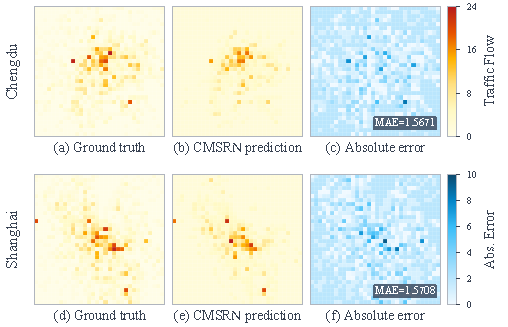
\includegraphics[width=\linewidth]{figures/cmsrn-spatial-h6.pdf}
  \caption[H6空间预测案例]{\textbf{第6个预测步（提前30分钟）的空间预测案例。}上排（a）--（c）为成都2016年11月25日09:50，下排（d）--（f）为上海2016年8月25日20:20，依次展示真实流量、CMSRN预测和绝对误差。每幅图表示原始\(32\times32\)网格上单个5分钟时间片的流入量与流出量之和；两城市采用统一色标，右侧上、下色条分别对应总流量与绝对误差。图内MAE为该时间片总流量在全部1,024个网格上的平均绝对误差，表格指标则按流量通道在测试集的正目标位置上计算。案例依据误差与空间对比度事后选取，时间均为UTC+8。}
  \label{fig:cmsrn-spatial-h6}
\end{figure}

% 情景性能与两条残差通路的分析统一纳入5.2。
% !TeX root = ../main.tex
% !TeX encoding = UTF-8
% !TeX spellcheck = none
% 由05-main-results.tex加载，继续5.2的三级标题编号。
\subsubsection{不同常规模式偏离程度下的预测性能}\label{sec:scenario-performance}\label{sec:exp-scenarios}

总体指标与空间案例之外，分组评价进一步考察模型在常规模式偏离时的预测表现及残差作用。分析使用生成现有图件时锁定的模型，在成都和上海分别使用第118轮和第116轮的检查点。全部分组仅使用预测起点之前的12步观测，常规参考和分位数阈值由训练历史拟合后冻结；各方法共享测试窗口、组别及正目标值掩码。分组MAE在相应预测步的有效样本--网格位置上合并计算，批次补齐样本不参与统计。

对各网格和通道，以训练历史中同工作日/周末类型、同五分钟时间槽的流量中位数作为外部分析的常规参考。历史观测减去该参考后，除以按网格和通道从训练残差拟合的稳健尺度\(\max(1,1.4826\,\mathrm{MAD})\)，得到标准化残差；取历史12步残差绝对值的均值作为偏离分数。按训练分数的第50、80和95百分位数，将测试位置划分为Low、Moderate、High和Extreme四组。该外部分组参考用于解释预测结果，不改变模型输入、训练或检查点选择；分组细节见补充材料S1。

\begin{figure}[!htbp]
  \centering
  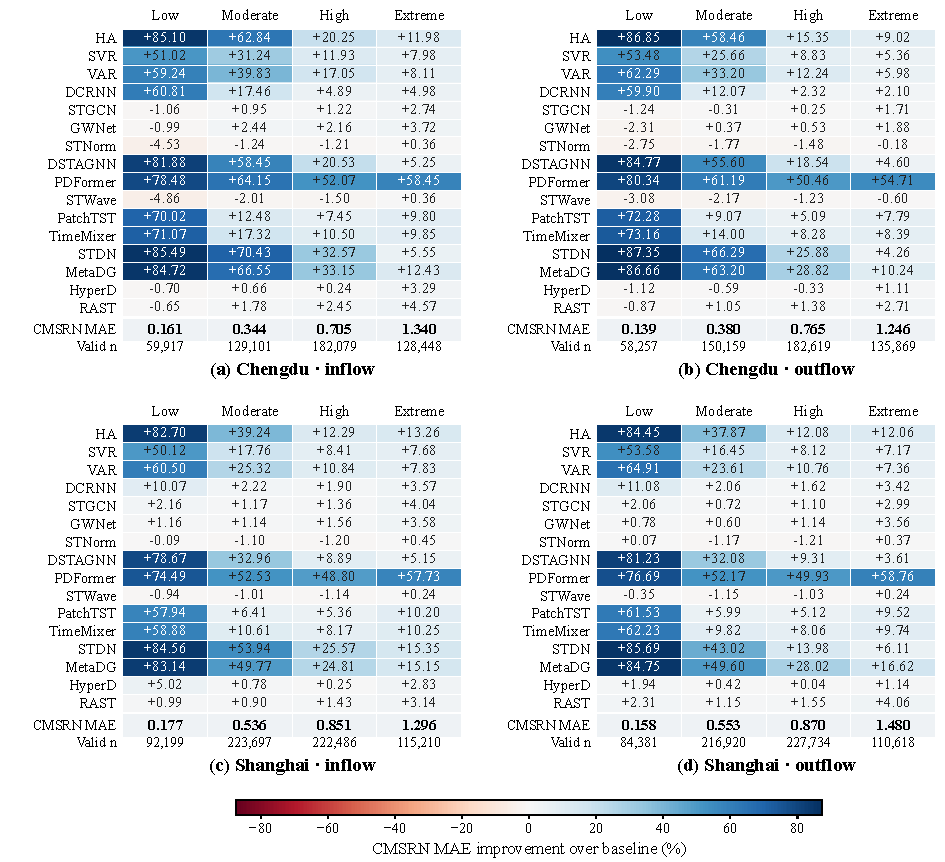
\includegraphics[width=\linewidth]{figures/scenarios/performance_h6_paper.pdf}
  \caption[常规模式偏离程度与H6预测性能]{\textbf{不同常规模式偏离程度下的H6预测性能。}四个面板对应成都和上海的流入、流出。单元格为\(100(\mathrm{MAE}_{m}-\mathrm{MAE}_{\mathrm{CMSRN}})/\mathrm{MAE}_{m}\)，正值（蓝色）表示CMSRN误差较低，负值（红色）表示相应基线误差较低。图中保留全部16种基线及统一色标；面板底部给出CMSRN的MAE和有效样本--网格数\(n\)。图内百分比保留两位小数。}
  \label{fig:scenario-performance}
\end{figure}

图~\ref{fig:scenario-performance}比较H6（提前30分钟）的分组表现。与总体结果表相比，情景分析另加入VAR、STNorm与STWave，构成16种基线的扩展比较。CMSRN在四项城市--通道任务中的MAE均随偏离等级升高而增大，但在Extreme组的相对排名更靠前：成都流入及上海两通道均排名第一，成都流出排名第三。前三项相对于最接近的基线STWave，MAE分别降低0.36\%、0.24\%和0.24\%；成都流出的MAE则比STWave高0.60\%。STNorm和STWave在多个较低偏离组中仍取得更低误差，表明CMSRN的相对竞争力具有情景和通道差异。

这一结果与本文关注局部流量偏离常规模式时的预测修正相呼应。与此同时，Extreme组的绝对误差仍较大，四项任务的MAE为Low组的7.32--9.38倍（补充图S1）。偏离等级还伴随流量规模变化，因此上述比较描述的是实际分组中的预测表现；其与残差通路的联系进一步由下述固定模型诊断考察。



\subsubsection{SERR在不同近期变化情景下的残差作用}\label{sec:scenario-serr}

在High与Extreme合并的高偏离子集中，以历史相邻标准化残差绝对差的均值描述近期变化强度，并按训练高偏离样本中该量的第75百分位数划分平缓变化（Slow）与快速变化（Rapid）两组。为考察已训练模型中各残差的实际作用，固定模型参数、门控和其余输出，分别从最终预测中扣除指定残差，计算
\begin{equation}
  \Delta\mathrm{MAE}_{e}
  =\mathrm{MAE}(\widehat Y-C_e)-\mathrm{MAE}(\widehat Y),
  \label{eq:scenario-residual-removal}
\end{equation}
其中\(C_e\)为实际加入预测的有符号修正量，包含门控、强度系数及逆标准化尺度。正值表示原残差降低了该组的平均MAE。该诊断与第\ref{sec:exp-ablation}节的独立重训练消融互为补充：前者度量锁定模型对既有修正的敏感性，后者比较重新训练后的修正通路配置。

图~\ref{fig:scenario-serr}中，两类专家在八个城市--通道--变化组上的16个移除差值均为正。自身残差在快速变化组的移除代价一致更大，为平缓组的1.61--2.82倍；例如，成都流入由0.0317增至0.0893，上海流入由0.0682增至0.1448。这说明，在当前高偏离样本中，节点自身演化修正在近期变化较快时对应更大的绝对MAE收益。时滞残差提供幅度较小的正向补充，其移除代价在成都的快速变化组增大，在上海则减小。两类角色呈现不同的情景响应，支持对自身动态与跨区域时滞信息分别组织修正证据。

\begin{figure}[!htbp]
  \centering
  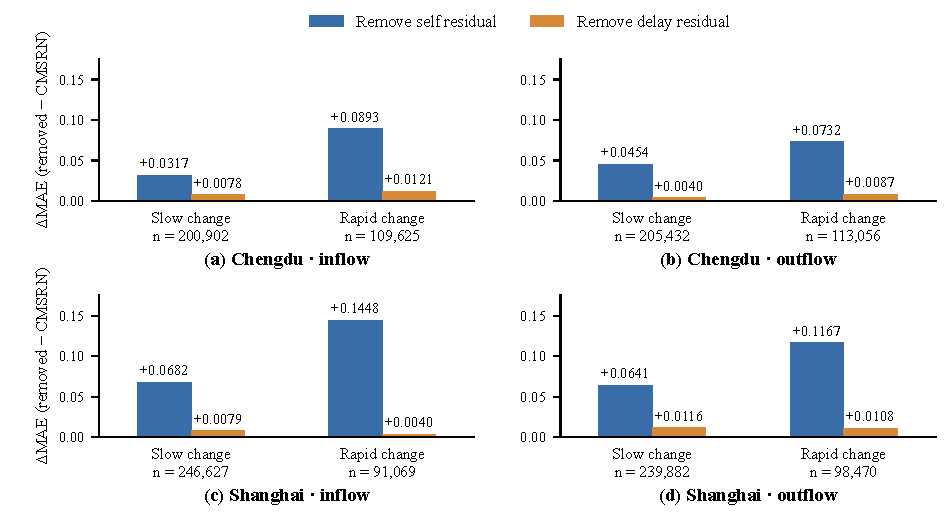
\includegraphics[width=0.92\linewidth]{figures/scenarios/serr_sensitivity_h6_paper.pdf}
  \caption[SERR在近期变化分组中的残差作用]{\textbf{高偏离情景下SERR的H6残差移除敏感性。}蓝柱和橙柱分别表示扣除自身残差与时滞残差后的\(\Delta\mathrm{MAE}\)，单位为原始5分钟流量计数；\(n\)为各组正目标样本--网格数。自身项扣除的是已加权的“自身预测减基础预测”修正。门控及其他残差保持不变，权重不重新归一化；两柱的MAE差值不具有可加性。}
  \label{fig:scenario-serr}
\end{figure}

\subsubsection{BCMS在不同背景差异与预测时距下的残差作用}\label{sec:scenario-bcms}

进一步在高偏离子集中，计算目标网格与各有效固定候选网格的历史平均标准化残差之差的绝对值，再对候选取均值，作为候选背景差异。使用训练高偏离样本的三分位阈值划分Low、Medium和High三组。该量由历史流量构造，是分析用的背景代理，并非BCMS内部学习到的低频表征。沿用式~\eqref{eq:scenario-residual-removal}，在H1--H12分别扣除完整BCMS修正，检查其作用随背景条件与预测时距的变化。

图~\ref{fig:scenario-bcms}显示，对每个城市、通道和预测步，低背景差异组的平均修正收益均高于中等组，中等组又高于高差异组。例如，上海流入在H6的三个\(\Delta\mathrm{MAE}\)依次为0.012448、0.008885和0.006301。144个背景组--预测步单元中有143个为正，唯一负值为成都流出高背景差异组H5的约\(-4.8\times10^{-6}\)。各组收益随预测步波动，未呈现随时距单调增加的规律。这些结果表明，BCMS的平均修正作用与候选背景条件有关，并在背景代理较接近的样本中更大。

将分析扩展至完整测试集后，各对应背景组--预测步的平均收益均高于高偏离子集，且仍保持低差异组高于中、高差异组的顺序（补充图S2）。例如，上海流入低背景差异组H6的\(\Delta\mathrm{MAE}\)由0.012448增至0.023927，表明BCMS的有效补充也覆盖其他交通状态。结合SERR的分组响应，自身演化修正在快速变化样本中具有更大的绝对MAE收益，而跨区域消息补充在背景代理较接近的样本中更有效。

\begin{figure}[!htbp]
  \centering
  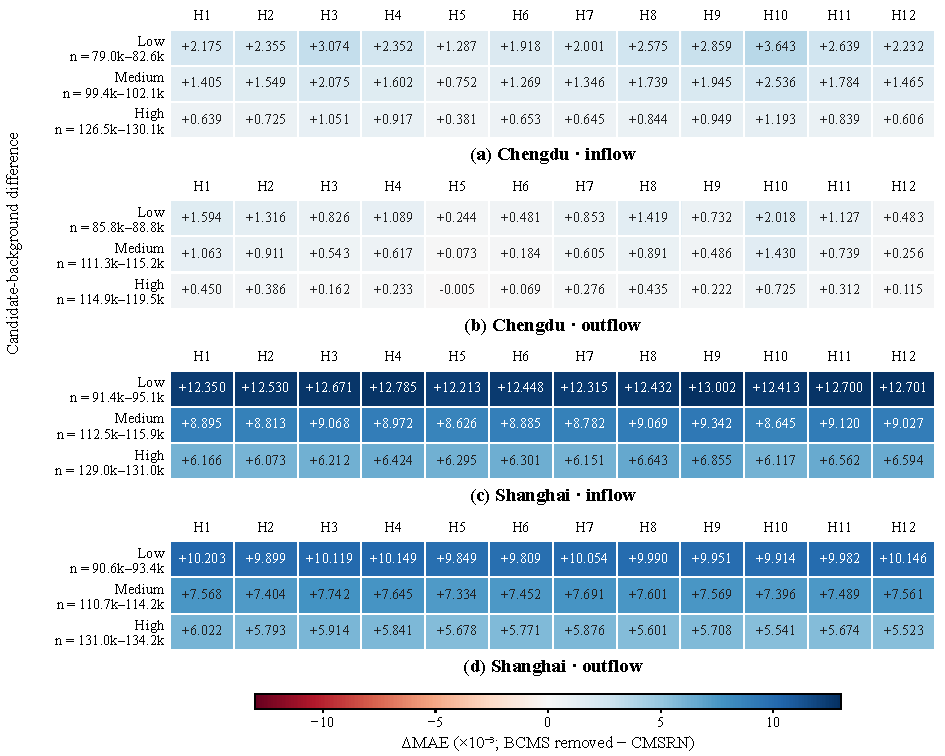
\includegraphics[width=0.92\linewidth]{figures/scenarios/bcms_sensitivity_horizons_paper.pdf}
  \caption[BCMS在背景差异与预测步分组中的残差作用]{\textbf{高偏离情景下BCMS的背景差异--预测步敏感性。}每格表示固定其余输出后扣除BCMS残差引起的MAE变化，数值按\(10^{-3}\)为单位显示，即图示值为\(1000\times\Delta\mathrm{MAE}\)。正值表示原修正降低组平均误差；H1--H12对应5--60分钟。背景组跨预测步保持固定，\(n\)的范围来自各步正目标位置数量的变化。该图为固定模型的输出移除诊断。}
  \label{fig:scenario-bcms}
\end{figure}



% !TeX root = ../main.tex
% !TeX encoding = UTF-8
% !TeX spellcheck = none
\subsection{消融实验}\label{sec:exp-ablation}

为评估各修正通路的贡献，我们在成都T5数据集上构建三种消融变体：去除自身专家的A1、去除有向时滞专家的A2，以及去除BCMS的A3。各变体均独立重新训练。对于A1与A2，被移除专家的门控权重置零，剩余专家的权重归一化为1。测试沿用第\ref{sec:exp-baselines-metrics}节的正目标值掩码与AVG12统计口径，以流入、流出指标的等权平均衡量整体预测性能；分通道结果见补充材料S4。

表~\ref{tab:serr-expert-ablation}显示，完整CMSRN在联合MAE和联合RMSE上均取得最低误差，三种消融变体则呈现不同的性能变化。去除自身专家后，联合MAE增加0.386\%，为三种变体中的最大增幅，同时联合RMSE增加0.301\%。这一结果说明，节点自身时序演化为基础预测提供了重要的修正依据，对降低整体平均误差具有较大贡献。

去除有向时滞专家后，联合MAE增加0.044\%，联合RMSE增加0.362\%，后者为三种变体中的最大增幅。考虑到RMSE对较大误差更敏感，这一差异表明，时滞关联的价值更多体现在对较大预测偏差的修正上。自身专家与时滞专家在两项指标上呈现不同的贡献特点，支持分别组织节点自身动态与跨区域滞后信息，并通过门控融合形成互补修正。

去除BCMS后，联合MAE和联合RMSE分别增加0.005\%和0.064\%。相较于两类专家，BCMS在全测试集平均指标上提供了较小的增益。结合第\ref{sec:scenario-bcms}节的背景差异分组分析，其作用进一步体现为随交通背景变化的历史消息补充。因此，消融结果与情景分析从整体性能和条件响应两个层面共同支持了模型设计：SERR组织自身演化与有向时滞证据，BCMS在此基础上提供背景条件化的进一步修正。

% !TeX root = ../main.tex
\begin{table}[!htbp]
  \centering
  \caption{成都T5数据集上的消融测试结果}
  \label{tab:serr-expert-ablation}
  \begingroup
  \linespread{1}\fontsize{10}{12}\selectfont
  \setlength{\tabcolsep}{5pt}
  \renewcommand{\arraystretch}{1.05}
  \begin{tabular*}{\linewidth}{@{\extracolsep{\fill}}lrrrr@{}}
    \toprule
    模型配置 & 联合MAE$\downarrow$ & 相对变化 & 联合RMSE$\downarrow$ & 相对变化 \\
    \midrule
    CMSRN & \textbf{0.708537} & --- & \textbf{1.258507} & --- \\
    w/o Self Expert (A1) & 0.711270 & +0.386\% & 1.262301 & +0.301\% \\
    w/o Delay Expert (A2) & 0.708852 & +0.044\% & 1.263068 & +0.362\% \\
    w/o BCMS (A3) & 0.708570 & +0.005\% & 1.259318 & +0.064\% \\
    \bottomrule
  \end{tabular*}
  \par\vspace{3pt}
  \begin{minipage}{\linewidth}
  \footnotesize
  注：各变体均独立重新训练。联合指标为流入、流出AVG12指标的等权平均；相对变化以完整CMSRN的对应指标为参照，正值表示误差增加。加粗表示列内最低误差。
  \end{minipage}
  \endgroup
\end{table}

\FloatBarrier


% !TeX root = ../main.tex
% !TeX encoding = UTF-8
% !TeX spellcheck = none
\subsection{超参数敏感性分析}\label{sec:exp-hyperparameters}

我们在成都数据集上开展单变量验证集敏感性实验，考察SERR门控隐藏维度、BCMS内部表征维度，以及两条残差通路的初始化参数。两个维度均在\(\{8,16,32,64,128\}\)中取值，\(\alpha_0\)与\(\beta_0\)均在\(\{0,0.001,0.01,0.05,0.1\}\)中取值。参考配置沿用主要对比实验的默认值\((32,32,0,0)\)，每次仅改变其中一个参数，其余设置保持不变。

验证指标采用正目标值掩码。在每个验证批次内，将样本、网格和12个预测步中的有效位置合并，分别计算流入与流出的MAE和RMSE；对两通道指标等权平均得到批次联合指标，再对各验证批次等权平均。成都的1,724个验证窗口补齐为1,728个窗口，以27个批次参与计算，4个补齐的重复窗口保留在统计中。本节报告上述批次平均验证误差，与第\ref{sec:exp-baselines-metrics}节测试集AVG12的汇总口径不同。

\begin{figure}[!htbp]
  \centering
  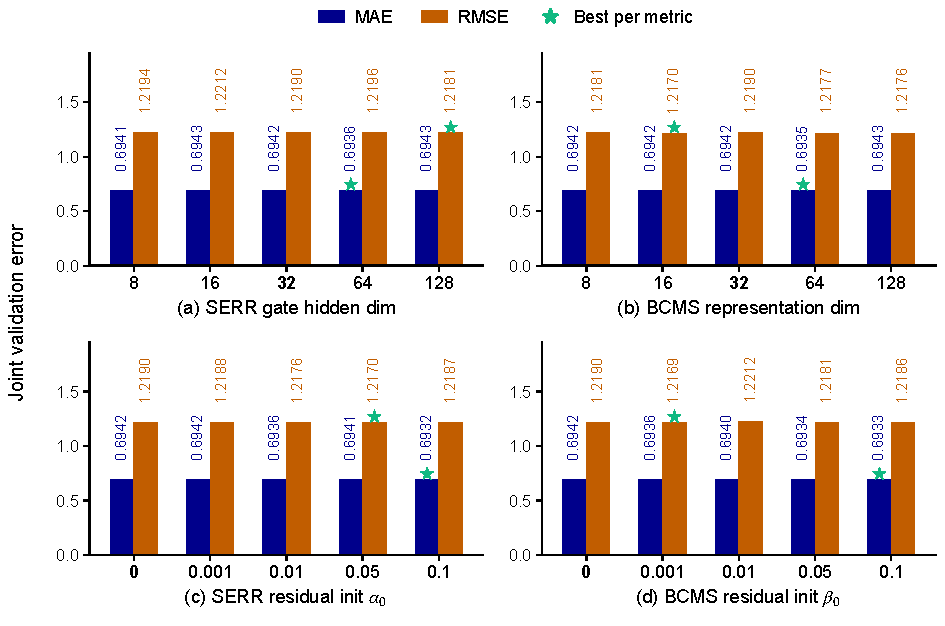
\includegraphics[width=\linewidth]{figures/hyperparameter-joint.pdf}
  \caption[联合验证指标的超参数敏感性]{\textbf{成都数据集上联合验证指标的超参数敏感性。}（a）SERR门控隐藏维度；（b）BCMS内部表征维度；（c）SERR残差强度初值\(\alpha_0\)；（d）BCMS残差参数初值\(\beta_0\)。蓝色和橙色柱分别对应MAE和RMSE，绿色星号标记每组中各指标的最小值，加粗横轴刻度表示参考配置；柱上数值保留四位小数，星号依据未舍入值确定。指标按正文所述验证批次口径汇总，联合指标对流入和流出等权平均。每个配置为固定种子42的一次运行，两项指标均在最低联合验证MAE所选检查点上计算。}
  \label{fig:hyperparameter-joint}
\end{figure}

图~\ref{fig:hyperparameter-joint}展示四组参数对应的联合验证误差。以每组最大与最小误差之差除以参考配置误差，四组联合MAE的相对极差均低于0.15\%，联合RMSE的相对极差均低于0.35\%。因此，在本次扫描范围内，四个参数的调整仅引起较小的验证误差变化。

隐藏维度的增大未带来单调改善。SERR门控隐藏维度为64时取得该组最低联合MAE，而最低联合RMSE出现在128；BCMS表征维度的对应最优值则分别为64和16。不同指标偏好的维度并不一致，较宽的内部表示也未在两项指标上形成持续优势。

残差初值直接赋给可学习参数，即\(\alpha(0)=\alpha_0\)、\(\beta(0)=\beta_0\)，其中BCMS的初始有效系数为\(\tanh(\beta_0)\)；两参数随后均参与训练。\(\alpha_0\)和\(\beta_0\)均在0.1时取得各自组内最低联合MAE，分别为0.693224和0.693278；最低联合RMSE则分别出现在\(\alpha_0=0.05\)和\(\beta_0=0.001\)。这些最小值与零初始化参考配置之间的差异较小，说明本次扫描中的组内最佳取值随评价指标而变化。

图~\ref{fig:hyperparameter-flow}进一步给出流入与流出的分通道结果。以SERR门控为例，流入MAE和RMSE的最优维度分别为64和128，而流出的两项指标均在维度8时最小；BCMS维度64则同时取得流出MAE和RMSE的最小值。这表明联合指标中的小幅变化仍包含通道间的不同响应，超参数比较应同时关注整体误差与分通道表现。



\begin{figure}[!htbp]
  \centering
  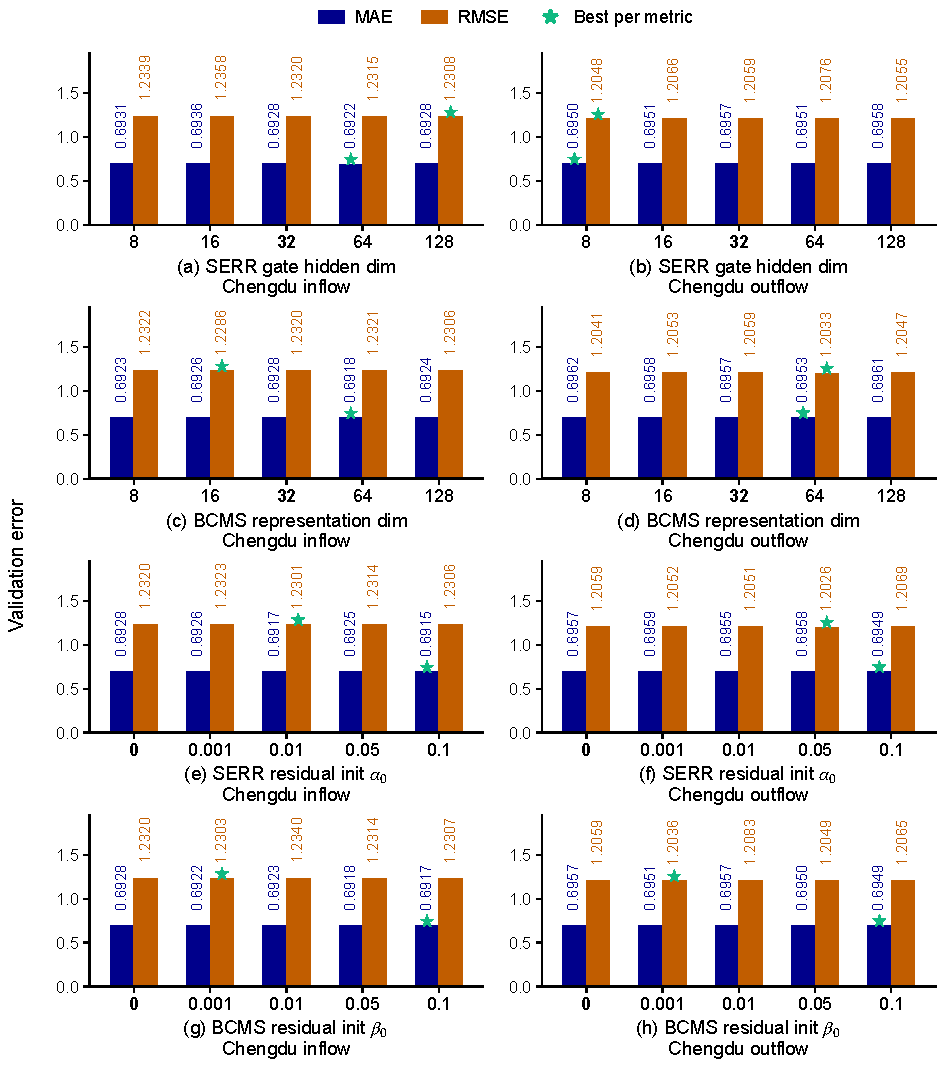
\includegraphics[width=\linewidth]{figures/hyperparameter-flow.pdf}
  \caption[流入与流出的超参数敏感性]{\textbf{成都数据集上流入与流出的超参数敏感性。}左列为流入，右列为流出；四行依次对应SERR门控隐藏维度、BCMS内部表征维度、\(\alpha_0\)和\(\beta_0\)。蓝色和橙色柱分别表示各通道按验证批次等权平均的MAE与RMSE，绿色星号标记组内最小值。参考刻度与数值显示规则同图~\ref{fig:hyperparameter-joint}。}
  \label{fig:hyperparameter-flow}
\end{figure}




% !TeX root = ../main.tex
% !TeX encoding = UTF-8
% !TeX spellcheck = none

\section{讨论}\label{sec:discussion}

CMSRN围绕常规流量模式偏离时的预测修正，将异质证据组织与历史消息选择纳入共享双频表征之上的残差框架。SERR按自身演化和有向时滞两类角色组织证据，BCMS依据流量背景与预测时距选择跨区域历史消息。两者从共享表征分别生成修正并作用于预测端，使不同来源的信息能够以明确的功能分工参与多步预测。

总体结果与情景分析共同说明，这一设计的预测优势具有状态和任务差异。在主要实验的13种基线范围内，CMSRN在两城市的流入、流出任务上均取得最低AVG12 MAE，相对最强基线降低0.46\%--2.00\%；其中成都流入的AVG12 RMSE降低5.01\%，上海流出的AVG12 RMSE则略高于最强基线。加入STNorm和STWave的扩展比较进一步显示，CMSRN在四项任务中的三项Extreme组取得最低MAE，而多个较低偏离组仍由上述强基线取得更低误差。这表明，整体误差、局部偏离程度与流量通道需要结合评价。空间案例中保留主要热点位置但存在幅值偏差的现象，也提示区域调度应用应同时关注流量分布与局部峰值误差。

两条残差通路的分组响应为理解这种差异提供了依据。自身修正在近期快速变化的高偏离样本中对应更大的绝对MAE收益，时滞修正提供幅度较小、随城市而变化的补充；BCMS的平均收益则在目标与候选背景代理较接近时更大，并覆盖高偏离子集之外的交通状态。这些观察支持将局部演化证据与跨区域历史信息分工处理，也表明跨区域补充的作用范围不限于强偏离情景。第\ref{sec:exp-ablation}节的独立重训练消融评价各修正通路的整体贡献，固定输出诊断则解释完整模型对既有残差的依赖，两类证据从不同角度刻画了角色修正的作用。

本研究在成都和上海各一个月的规则网格数据上，考察了CMSRN对5–60分钟交通流量的预测能力。现有实验主要反映观测时段内的短时预测表现，其在跨季节变化和持续性交通模式迁移下的适应能力值得进一步研究。当前常规参照、有向时滞关系与候选支持在预测阶段保持固定，如何随交通状态演变更新这些先验信息，是拓展模型时间适应性的关键。

未来研究将进一步探索时间适应性。面向更长时间跨度的交通变化，研究常规参照、有向时滞关系与候选支持的动态更新，使预测修正能够持续适应周期规律和跨区域关联的演变。在此基础上，结合预测目标严格隔离的评估，以及对零流量区域和局部峰值的分析，进一步检验模型在不同流量状态下的适用性，为持续变化的交通环境提供更可靠的短时预测支持。


\FloatBarrier
% !TeX root = main.tex
% !TeX spellcheck = none
% 文献信息与排列顺序照录原稿；未补造或在线核验。
\begingroup
\linespread{1.05}\selectfont
\begin{thebibliography}{99}
\setlength{\itemsep}{3pt}
\bibitem{ref01}
Y. Li, R. Yu, C. Shahabi, and Y. Liu, ``Diffusion convolutional recurrent neural network: Data-driven traffic forecasting,'' in \emph{Proc. Int. Conf. Learn. Represent. (ICLR)}, 2018.

\bibitem{ref02}
B. Yu, H. Yin, and Z. Zhu, ``Spatio-temporal graph convolutional networks: A deep learning framework for traffic forecasting,'' in \emph{Proc. 27th Int. Joint Conf. Artif. Intell. (IJCAI)}, 2018, pp. 3634--3640.

\bibitem{ref03}
Z. Wu, S. Pan, G. Long, J. Jiang, and C. Zhang, ``Graph WaveNet for deep spatial-temporal graph modeling,'' in \emph{Proc. 28th Int. Joint Conf. Artif. Intell. (IJCAI)}, 2019, pp. 1907--1913.

\bibitem{ref04}
S. Guo, Y. Lin, N. Feng, C. Song, and H. Wan, ``Attention based spatial-temporal graph convolutional networks for traffic flow forecasting,'' in \emph{Proc. AAAI Conf. Artif. Intell.}, vol. 33, no. 1, 2019, pp. 922--929.

\bibitem{ref05}
C. Zheng, X. Fan, C. Wang, and J. Qi, ``GMAN: A graph multi-attention network for traffic prediction,'' in \emph{Proc. AAAI Conf. Artif. Intell.}, vol. 34, no. 1, 2020, pp. 1234--1241.

\bibitem{ref06}
Z. Wu, S. Pan, G. Long, J. Jiang, X. Chang, and C. Zhang, ``Connecting the dots: Multivariate time series forecasting with graph neural networks,'' in \emph{Proc. 26th ACM SIGKDD Int. Conf. Knowl. Discovery Data Mining (KDD)}, 2020, pp. 753--763.

\bibitem{ref07}
L. Bai, L. Yao, C. Li, X. Wang, and C. Wang, ``Adaptive graph convolutional recurrent network for traffic forecasting,'' in \emph{Adv. Neural Inf. Process. Syst. (NeurIPS)}, vol. 33, 2020, pp. 17804--17815.

\bibitem{ref08}
C. Song, Y. Lin, S. Guo, and H. Wan, ``Spatial-temporal synchronous graph convolutional networks: A new framework for spatial-temporal network data forecasting,'' in \emph{Proc. AAAI Conf. Artif. Intell.}, vol. 34, no. 1, 2020, pp. 914--921.

\bibitem{ref09}
M. Li and Z. Zhu, ``Spatial-temporal fusion graph neural networks for traffic flow forecasting,'' in \emph{Proc. AAAI Conf. Artif. Intell.}, vol. 35, no. 5, 2021, pp. 4189--4196.

\bibitem{ref10}
J. Jiang, C. Han, W. X. Zhao, and J. Wang, ``PDFormer: Propagation delay-aware dynamic long-range Transformer for traffic flow prediction,'' in \emph{Proc. AAAI Conf. Artif. Intell.}, vol. 37, no. 4, 2023, pp. 4365--4373.

\bibitem{ref11}
Y. Fang, Y. Qin, H. Luo, F. Zhao, B. Xu, L. Zeng, and C. Wang, ``When spatio-temporal meet wavelets: Disentangled traffic forecasting via efficient spectral graph attention networks,'' in \emph{Proc. IEEE 39th Int. Conf. Data Eng. (ICDE)}, 2023, pp. 517--529.

\bibitem{ref12}
Y. Nie, N. H. Nguyen, P. Sinthong, and J. Kalagnanam, ``A time series is worth 64 words: Long-term forecasting with Transformers,'' in \emph{Proc. Int. Conf. Learn. Represent. (ICLR)}, 2023.

\bibitem{ref13}
S. Wang, H. Wu, X. Shi, T. Hu, H. Luo, L. Ma, J. Y. Zhang, and J. Zhou, ``TimeMixer: Decomposable multiscale mixing for time series forecasting,'' in \emph{Proc. Int. Conf. Learn. Represent. (ICLR)}, 2024.

\bibitem{ref14}
J. Zhang, Y. Zheng, and D. Qi, ``Deep spatio-temporal residual networks for citywide crowd flows prediction,'' in \emph{Proc. AAAI Conf. Artif. Intell.}, vol. 31, no. 1, 2017, pp. 1655--1661.

\bibitem{ref15}
Z. Lin, J. Feng, Z. Lu, Y. Li, and D. Jin, ``DeepSTN+: Context-aware spatial-temporal neural network for crowd flow prediction in metropolis,'' in \emph{Proc. AAAI Conf. Artif. Intell.}, vol. 33, no. 1, 2019, pp. 1020--1027.

\bibitem{ref16}
D. A. Tedjopurnomo, Z. Bao, B. Zheng, F. M. Choudhury, and A. K. Qin, ``A survey on modern deep neural network for traffic prediction: Trends, methods and challenges,'' \emph{IEEE Trans. Knowl. Data Eng.}, vol. 34, no. 4, pp. 1544--1561, Apr. 2022.

\bibitem{ref17}
W. Jiang, J. Luo, M. He, and W. Gu, ``Graph neural network for traffic forecasting: The research progress,'' \emph{ISPRS Int. J. Geo-Inf.}, vol. 12, no. 3, Art. no. 100, 2023.

\bibitem{ref18}
Y. Xu, L. Wei, and L. Feng, ``A spatial-temporal trend-event decoupling dual-channel framework for traffic flow prediction,'' \emph{Expert Syst. Appl.}, vol. 287, Art. no. 128107, 2025.
% 本节新增基线文献已核对PMLR/AAAI官方页面，2026-10-26。
\bibitem{ref19}
S. Lan, Y. Ma, W. Huang, W. Wang, H. Yang, and P. Li,
``DSTAGNN: Dynamic spatial-temporal aware graph neural network for traffic flow forecasting,''
in \emph{Proc. 39th Int. Conf. Mach. Learn. (ICML)},
vol. 162, 2022, pp. 11906--11917.

\bibitem{ref20}
L. Cao, B. Wang, G. Jiang, Y. Yu, and J. Dong,
``Spatiotemporal-aware trend-seasonality decomposition network for traffic flow forecasting,''
in \emph{Proc. AAAI Conf. Artif. Intell.},
vol. 39, no. 11, 2025, pp. 11463--11471,
doi: 10.1609/aaai.v39i11.33247.

\bibitem{ref21}
Y. Zou, H. Yuan, Q. Yang, Z. Yuan, S. Wang, and S. Ruan,
``Meta dynamic graph for traffic flow prediction,''
in \emph{Proc. AAAI Conf. Artif. Intell.},
vol. 40, no. 19, 2026, pp. 16584--16592,
doi: 10.1609/aaai.v40i19.38699.

\bibitem{ref22}
M. Shao, Z. Zhang, Y. Wang, Y. Dai, X. Shen, and X. Wang,
``HyperD: Hybrid periodicity decoupling framework for traffic forecasting,''
in \emph{Proc. AAAI Conf. Artif. Intell.},
vol. 40, no. 18, 2026, pp. 15689--15697,
doi: 10.1609/aaai.v40i18.38599.

\bibitem{ref23}
W. Ruan, X. Dang, Z. Zhou, S. Lyu, and Y. Liang,
``A retrieval augmented spatio-temporal framework for traffic prediction,''
in \emph{Proc. AAAI Conf. Artif. Intell.},
vol. 40, no. 46, 2026, pp. 39163--39172,
doi: 10.1609/aaai.v40i46.41264.

% 情景扩展基线：核对ACM出版记录，2026-10-27。
\bibitem{ref24}
J. Deng, X. Chen, R. Jiang, X. Song, and I. W. Tsang,
``ST-Norm: Spatial and temporal normalization for multi-variate time series forecasting,''
in \emph{Proc. 27th ACM SIGKDD Conf. Knowl. Discov. Data Min. (KDD)},
2021, pp. 269--278, doi: 10.1145/3447548.3467330.

\end{thebibliography}
\endgroup

\end{document}
